
\documentclass[12pt]{article}
\usepackage{amsmath}
\usepackage{graphicx}
\usepackage{natbib}
\usepackage{url}
\usepackage{blkarray}

\newcommand{\blind}{0}

\addtolength{\oddsidemargin}{-.5in}
\addtolength{\evensidemargin}{-1in}
\addtolength{\textwidth}{1in}
\addtolength{\textheight}{1.7in}
\addtolength{\topmargin}{-1in}

\input{Header}
\setcitestyle{numbers,square}
\begin{document}


\def\spacingset#1{\renewcommand{\baselinestretch}
{#1}\small\normalsize} \spacingset{1}



{
	\title{\bf Knowledge Transfer in High-Dimensional Heterogeneous Time Series Via Moderators}
	\author{
		José Á. Sánchez Gómez \and  Holly O'Rourke \and  Gene Brewer \thanks{ José Á. Sánchez Gómez is Assistant Professor, Department of Statistics, University of California Riverside, Riverside, CA 92521, USA. E-mail: \href{mailto:josesa@ucr.edu}{josesa@ucr.edu}. Holly O'Rourke is Associate Professor, Department of Psychology, University of California Riverside, Riverside, CA 92521, USA. Email: \href{mailto:holly.orourke@ucr.edu}{holly.orourke@ucr.edu}. Gene Brewer is Professor, Department of Psychology, University of California Riverside, Riverside, CA 92521, USA.\\
		Corresponding Authors: José Á. Sánchez Gómez (\href{mailto:josesa@ucr.edu}{josesa@ucr.edu}), Holly O'Rourke (\href{mailto:holly.orourke@ucr.edu}{holly.orourke@ucr.edu}).}
	}
	\date{}
	\maketitle
}


\bigskip
\begin{abstract}
	In psychological research, there is a growing interest in the quantification of both nomothetic and idiographic variation in human behavior. This is especially pressing in the analysis of intensive longitudinal data for multiple subjects, where there is interest in understanding both inter-subject and intra-subject variability for a set of $d$ variables evolving over time. Often, researchers measure a set of $p$ additional time-invariant moderators, which further describe the subjects in the study.  Although several methods have been recently proposed for the simultaneous estimation of common and individual components of variation for longitudinal data, they are not designed to incorporate the information of the time-invariant moderators, which may have a role in the intra-subject variability. Current methods that may incorporate moderator variables are not properly equipped to handle high-dimensionality when the number of variables of interest $d$ and moderator variables $p$ are large. In this paper, we propose the MOD-VAR method, that efficiently estimates the presence of common variation across subjects, as well as individual variability explained by underlying moderator variables of interest. We provide numerical simulations that confirm the superior performance of our proposed MOD-VAR with methods in the literature in terms of network recovery and forecasting accuracy. Our theoretical guarantees show that our proposed MOD-VAR method estimates both the joint and individual network connections consistently, even for limited number of subjects $n$ and measured time points $T$, as long as $ nT \gtrsim \log(pd)$. Finally, we exemplify the use of our proposed MOD-VAR on a longitudinal study of human behavior, and study the effect that moderators like gender or employment have on the dynamics of anxiety, depression, and sleep. 
\end{abstract}

\noindent
{\it Keywords:}  \jose{add}
\vfill


\newpage
\spacingset{1.5}
\setlength{\abovedisplayskip}{2pt}
\setlength{\belowdisplayskip}{2pt}






\section{Introduction}

\jose{CONCEPTS TO ADD?}
\begin{itemize}
	\item \jose{The idea that previous methods to incorporate external data are focused on modeling the effect that external variables have on the mean behavior, not on the actual structure of the parameters. In this sense, our analysis is deeper.}
	\item \jose{Pivot the narrative to think about contextual transfer learning: we are transfering knowledge across the graphs, but we are doing so by also incorporating context into our estimation. This allows for a more nuanced estimation, where we can explain some of the heterogeneity and deviation from the base model by relevant factors.}
\end{itemize}

%% Intro to time series analysis and recent works. 
The modeling and forecasting of intensive multivariate time series data has been a long-standing area of research in statistics, optimization and machine learning \jose{(cite)}, with applications in economics, finance, neuroscience and psychology \jose{(cite)}, among other areas. In particular, researchers are often interested in constructing a \textit{Granger-causal network} (GCN) to describe the dependence that variables in the time series have over time. In a GCN, nodes correspond to variables in the time series, and a directed link between two nodes represents an effect of the origin variable in the present to future values of the target variable. When the time dependence is linear, the GCN can be fully recovered by estimating coefficients of a sparse vector auto-regressive model (VAR). This has been the subject of a wide variety of studies. \jose{(cite)}. As a consequence, a wide variety of methods have been developed for the reliable estimation of GC networks for high-dimensional time series data \jose{(cite)}. For a review, see \jose{(cite)}.

%% Introduction of the problem: multi subject time series with 
One major statistical challenge is that of estimating GCNs over multiple subjects. For example, in fMRI studies, often researchers are interested in determining the patterns of communication among different regions of the brain. By processing functional magnetic resonance imaging (fMRI) data, researchers can measure the activity of different brain regions over time. Thus, a GCN may describe the connectivity of electrical signals across different brain regions. In studies with data measured multiple subjects, we expect the connectivity patterns to be heterogeneous, with the presence and intensity of connections in the GCNs varying across individuals. Despite this, it is expected that many baseline connections are common and similar across subjects. In this case, fitting a single VAR model may lead to bias and inaccurate forecasting. On the other hand, training separate VAR models for each subject may miss the chance to exploit the common structure to obtain improved forecasting accuracy.  

%% Summary of things that have been done in the consistent estimation of time series. 
Several works have explored the problem of fitting and testing models for multi-subject high dimensional GCNs. The Multi-VAR method \jose{(cite)} applies a penalized estimation to recover both joint and individual components of a GCN, validated with extensive numerical experiments.  On the other hand, GIMME is a . More recently, \jose{(cite)} develops a multiple testing procedure based on the debiased lasso \jose{(cite)} to determine if there are significant differences in the GCN across multiple subjects. 

%% Research gap: cannot explain the source of this heterogeneity.
Prior works have successfully modeled heterogeneous time series data across multiple subjects. Despite this progress, a key question remains unanswered: \textit{can we explain the source of this heterogeneity across multiple subjects?} For example, in the aforementioned fMRI study, researchers may be interested not only in detecting heterogeneity in the GCN across individuals, but to determine the influence that external factors like age, gender, and existing health conditions or  treatments may have in the inter-subject heterogeneity. While prior methods may measure this heterogeneity, they are ill-equipped to incorporate this additional external covariate-level information to inform the estimation of GCNs. 


% Multi-level: limitations
Models for relating VAR coefficients to additional time-invariant variables have been explored in the past, and belong to the area of multi-level VAR \jose{cite}. These methods have limited applicability in general, since they are are often unable to handle a large number of variables $d$ or moderator variables $p$ unless the number of subjects or time-measurements per subjects are prohibitively large. On the other hand, the X-VAR model incorporates the effect of external moderators to the VAR forecasting model \jose{(cite)}. Despite its advantages, the effect of the external moderators is considered only as an effect on the mean behavior of the time series, and therefore does not consider the potential effects that this moderators have on the GCN structure. Thus, there is a pressing need for methods that can estimate the influence that moderator variables have on the intra-subject variability of behavior, and can provide reliable estimates, even in cases where the number of parameters may be significantly larger than the number of observations. 



%% What do we do here? We introduce MOD-VAR, which estimates structure that is common, moderator dependent, and fully individual structure. We provide convergence guarantees and extensive simulations that confirm superior performance. 
In the present paper, we propose the moderator vector autoregressive model (MOD-VAR) for the simultaneous estimation of GCN over multiple heterogeneous time series, which measures the effect that external covariates may have on the each subject's GCN. Our method can thus quantify (\textit{i}) the GCN structure that is shared across all subjects, (\textit{ii}) the GCN that is dependent on external moderators, and (\textit{iii}) the connections in the GCN that are individual, and cannot be explained by the given moderator variables. Our method is highly general, encompassing the Multi-VAR framework \jose{(cite)}. 

%% Our contributions are two fold: we introduce method.
Our theoretical findings confirm that our proposed MOD-VAR can achieve consistent estimation of all parameters, as long as  $nT \gg \log(pd^2)$. Furthermore, we conduct extensive simulation scenarios, which show the improved performance of our proposed MOD-VAR when compared to other methods in the literature designed for the estimation of common and individual  components of GCNs for multiple subject longitudinal data. To showcase the usefulness of our method in real data applications, we analyze \jose{the daily emotional assessment dataset}, and show links between gender, employment status and the dynamics of depression, anxiety and sleep.  


% Our paper's order. 
The rest of the paper is organized as follows. In section \ref{section:mod-var} we introduce our model of moderator time series model, and introduce our MOD-VAR estimator. In section \ref{section:method} we provide details on the implementation of our proposed method. In Section \ref{section:simulations} we provide numerical comparisons of our proposed MOD-VAR with methods found in the literature. In Section \ref{section:realData} we exemplify the use of our MOD-VAR method in the analysis of daily mood and behavior psychological data. Closing remarks and discussions are found in Section \ref{section:discussion}


%\subsection*{Notational Conventions} 

We establish the following notational conventions. For any $n$, let $[n] = \{1,2,\ldots ,n\}$. For any $k\leq \ell$, we denote $[k : \ell] = \{k,k+1,\ldots, \ell-1, \ell\}$. For any $\Ar \in\bbR^{p\times q}$, we denote the transpose of $\Ar$ as $\Ar'$. For $\bx= (x_1,x_2,\ldots ,x_d)'\in\bbR^{d}$, we denote by $\|\bx\|_1, \|\bx\|_2, \|\bx\|_{\infty}$ the $\ell_1$-norm, euclidean norm and entrywise maximum norm respectively, given by $\|\bx\|_1 = \sum_{i=1}^d |x_i|$, $\|\bx\|_2 = \sqrt{\bx'\bx}$, and $\|\bx\|_\infty = \max_{i\in[d]} |x_i|$. For any $\Sigma= (\sigma_{ij})_{i,j=1}^d\in\bbR^{d\times d}$, we denote the trace as $\btr(\Sigma) = \sum_{i\in[d]} \sigma_{ii}$. For $\Ar \in\bbR^{p\times q}$, we denote by $\vertiii{\Ar}_2$, and $\vertiii{\Ar}_F$  the $\ell_2$ operator,  and Frobenius norms, respectively, given by $\vertiii{\Ar}_2 := \sup_{\bx\in\bbR^{q}\setminus\{\bzero\}} \|\Ar \bx\|_2 / \|\bx\|_2$, and $\vertiii{\Ar}_F = \sqrt{\btr(\Ar'\Ar)}$. Additionally, we denote by $\|\Ar\|_{1}$ the vectorized $\ell_1$-norm of the matrix $\Ar$, given by $\|\Ar\|_1 = \sum_{i,j}|A_{ij}|$. For any $k$, we denote $\indv{k}\in\bbR^{k}$ the vector with all one entries. For any set $A$, we denote by $\ind{A}$ the indicator function of $A$. For any $x\in\bbR$, we denote $\bsign(x) = \ind{x> 0} - \ind{x<0}$. For any symmetric matrix $\Sigma\in\bbR^{d\times d}$, we denote the minimum and maximum eigenvalues of $\Sigma$ as $\Lambda_{\min}(\Sigma),\Lambda_{\max}(\Sigma)\in\bbR$, respectively.


%%%%%%%%%%%%%%%%%%%%%%%%%%%%%%%%%%%%%%%%%%%%%%%%%%%%


\section{Moderator Vector Autoregressive Model}\label{section:mod-var}




\subsection{Vector Autoregressive Models}

Consider a longitudinal study with $n$ subjects. For each subject $k\in[n]$, we have access to the measurements of $d$ different variables of interest over $T_k$ equally spaced time points, which we denote by $\Yb_{k} = \{ \bY_{t}^{(k)} \}_{t = 1}^{T_k}\subset \bbR^{d}$. In this context, it is important to understand the lagged temporal relationships that exist between the different variables. This can be achieved via a VAR(1) model, which can be expressed as
\begin{equation*}
	\bY_{t}^{(k)} =  \Phi^{*(k)} \bY_{t-1}^{(k)} + \bvarepsilon_{t}^{(k)}, \hspace{5mm} \text{for all } 2\leq t\leq T_k,
\end{equation*}
where $\Phi^{*(k)}$ is a $d\times d$ matrix that represents the true lag-1 multivariate relationships for the subject $k$. In particular, for $1\leq i,j\leq d$, the entry $\Phi^{*(k)}_{ij}$ represents the effect that the variable $j$ at time $(t-1)$ affects the variable $i$ at time $t$. Notice that we define a distinct coefficient matrix $\Phi^{*(k)}$ for each subject $k\in[n]$. \jose{Mention how GCN is defined in terms of $\Phi$'s.}

When encountering a study with multiple subjects, there are several potential approaches to consider. A simple approach consists of simply assuming that all subjects have the same lagged temporal relationships, \textit{i.e.,} $\Phi^{*} := \Phi^{*(1)} = \Phi^{*(2)} =\ldots = \Phi^{*(n)} $.  Under this assumption, the estimation of $\Phi$ can be performed by pooling the data from all subjects and performing standard VAR estimation \jose{(cite)}. This approach exclusively focuses on the estimation of shared components on a GCN, and ignores the potential presence of individual-level heterogeneity. Alternatively, one may perform the estimation of each $\{\Phi^{*(1)}, \Phi^{*(2)}, \ldots , \Phi^{*(n)}\}$ separately, by fitting a different VAR model to each model. While this approach allows for the study of individual-level GCN structure, it does not exploit the potential common structure that is likely to be shared across most subjects. 

More recently, Multi-VAR \citet{fisher2022penalized} explores the estimation of multiple VAR models, allowing for the presence of both common and idividual components. To this end, they assume that the subject-level coefficients of the VAR(1) model satisfy the decomposition,
\begin{equation*}
	\Phi^{*(k)} = \Phi^{*(0)} + \bDelta^{*(k)},\hspace{5mm} \text{for all }k=1,\ldots, n.
\end{equation*}
where $\Phi^{*(0)}$ is a $d\times d$ matrix representing the coefficients common across all subjects, and $\bDelta^{*(k)}$ represents relationships exclusive to subject $k$.  While the multi-VAR model accounts for inter-subject structural variability, it only focuses on quantifying differences in the GCN, without studying the potential explanatory sources of said heterogeneity. Thus, there is an important question that remains unanswered: \textit{Can part of the inter-subject heterogeneity be explained by external moderator variables?} This question is at the core of our proposed methodology. 


\subsection{Moderator Vector Autoregressive Models}

For each subject $k=1,2,\ldots, n$, in addition to the time-series data $\Yb_k$, we have a set of $p$ potential moderator variables $\bX_k = (X_{k1}, X_{k2}, \ldots, X_{kp})'\in\bbR^{p}$. Notice that the moderators in $\bX_k$ are not time-varying, and thus can be thought as stable features of each subject. For example, in a neuroimaging study analyzing brain connectivity, these moderators may include clinical or demographic variables such as gender or age. We may also consider control experimental variables of interest such as treatment status of individual, or magnitude of the dose provided to a patient.

First, consider the scenario in which the cross-subject heterogeneity can be fully explained by the set of external moderators $\bX_k$. We can represent the moderator-dependent time series lagged relationships as $\Phi^{*(k)} = \Phi^{*}(\bX_k)$, where, for any vector of $p$ moderators $\bx = (x_1, x_2, \ldots , x_p)'$,
\begin{equation}\label{eq:mod_noIdiographic}
    \Phi^{*}(\bx) := \Phi^{*(0)} + x_1 \Phi^{*(M1)} + x_2 \Phi^{*(M1)} + \ldots + x_p \Phi^{*(Mp)} ,
\end{equation}
where $\Phi^{*(0)},\Phi^{*(M1)}, \Phi^{*(M2)}, \ldots, \Phi^{*(Mp)}\in\bbR^{d\times d}$. Similar to existing methods, $\Phi^{0}$ represents the shared connectivity in the GCN across subjects. For each moderator variable $1\leq \ell\leq p$, the matrix $\Phi^{(M\ell)}$ represents the effect that the $\ell$-th moderator has on the time series dynamic. More specifically, for $i,j\in[d]$ and $\ell\in[p]$ the entry $\Phi^{*(M\ell)}_{ij}$ represents the effect that the moderator variable $\ell$ has on the lagged relationship of $j$ on the variable $i$. In particular, if a subject has $x_{\ell}= 0$, then $x_{\ell} \Phi^{*(M\ell)} = \bzero$ and thus, the moderator $\ell$ does not have any effect on the multivariate time dynamics for this subject. In addition, the larger the value of $x_{\ell}$, the stronger the effect that the moderator $\ell$ have on the dynamic of the corresponding subject. 

Under the model \eqref{eq:mod_noIdiographic}, the time series dependence for subject $k$ can be written as,
\begin{equation}\label{eq:vareq_idiographic}
    \bY_{t}^{(k)} =  \Phi^*(\bX_k) \bY_{t-1}^{(k)} + \bvarepsilon_{t}^{(k)}, \hspace{5mm} \text{for all } 1\leq k\leq n \text{ and }2\leq t\leq T_k.
\end{equation}

\begin{ex}\label{ex:modvar_p2}
    We consider a VAR(1) model with $n$ subjects. For each subject, we measure two time-invariant moderators (\textit{i.e.,} $p = 2$). In that case, $\bX_k = (X_{k1},X_{k2})^{'}$. Then, the MOD-VAR model with 2 moderators is given by,
	\begin{align*}
		\bY^{(k)}_t &= \Phi(\bX_k) \bY_{t-1}^{(k)} + \be^{(k)}_{t}\\
		&= [\Phi^{*(0)} + X_{k1} \Phi^{*(M1)} + X_{k2} \Phi^{*(M2)}] \cdot \bY_{t-1}^{(k)} + \be^{(k)}_{t}
	\end{align*}
	Notice that the GCN of a subject $k\in[n]$ incorporates a a common structure shared across all subjects $\Phi^{*(0)}\in\bbR^{d\times d}$, and an individual structure. In contrast with prior works, the individual connections in the GCN have the form $X_{k1} \Phi^{*(M1)} + X_{k2} \Phi^{*(M2)}$, from which they depend on the information of our moderator variables $\bX_k = (X_{k1}, X_{k2})^{'}$ of each subject. A further description of this scenario can be found in Figure \ref{fig:rvarCoeffsExample}
\end{ex}
\begin{figure}
		\centering
		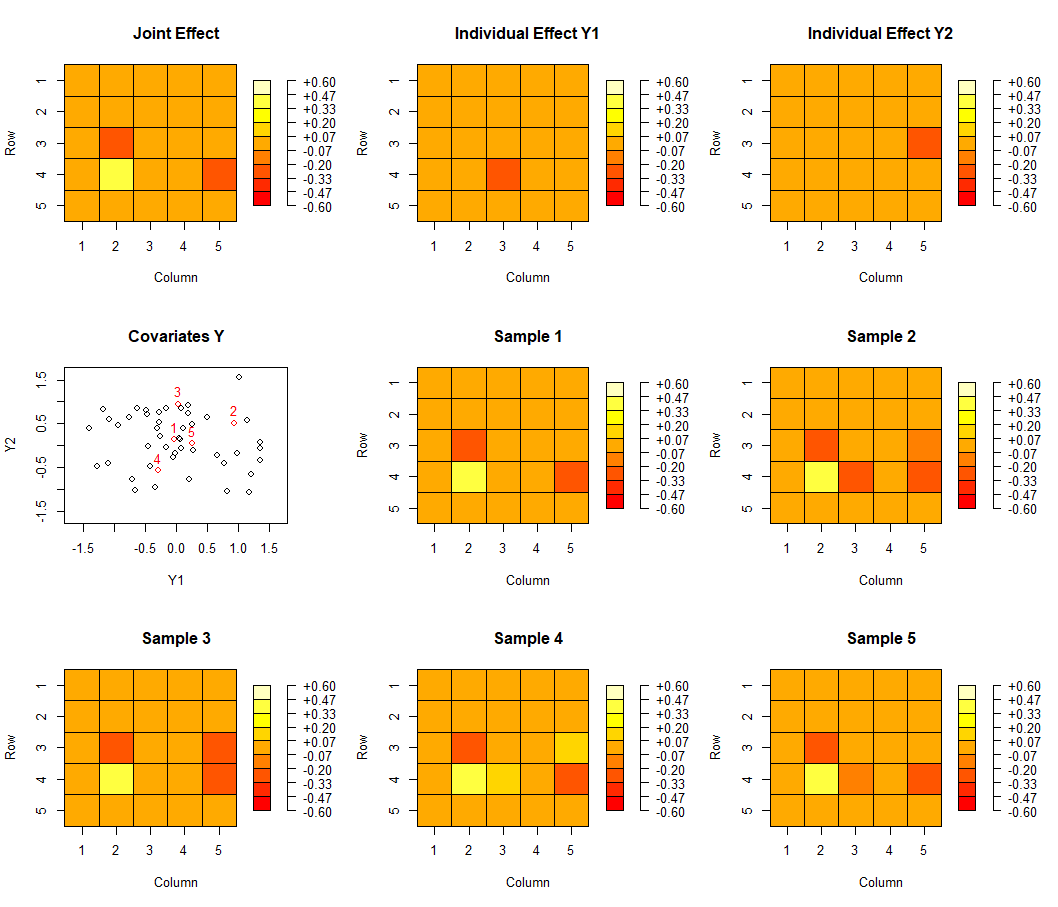
\includegraphics[width = \linewidth]{figures/1_VisParExample}
		\caption{Illustration of the Regression VAR framework with 2 covariate-dependent effects, as discussed in Example \ref{ex:modvar_p2}. Top-panels: visualization of the joint effects that are common across all subjects. We also visualize the effects that are individual to variables $X_1$ and $X_2$. Center-left panel: Visualization of the covariate information for $N = 50$ subjects. We highlight the covariate information of the first 5 subjects. Remaining panels: Visualization of the effects for the first 5 subjects. We observe that, as subject 1 has nearly zero for both $X_1$ and $X_2$, the effects are mostly just the joint effects. Subject 3 has a high $X_2$ covariate, but low $X_1$ covariate, and therefore its effects are a mixture of the joint and $X_2$ effects. Subject 2 has large covariates for both $X_1$ and $X_2$, so its time series effects are a mixture of all.}\label{fig:rvarCoeffsExample}
	\end{figure}


\subsection{Moderator Vector Autoregressive Models with Individual Remainders}


We may consider an additional scenario, in which moderator variables do not explain all cross-subject heterogeneity. In this case, in addition to a shared network across all individuals $\Phi{*}$, and moderator-related individual effects, there is an additional fully individual structure in our model. We consider, for each subject $k$, the coefficient matrix $\Phi^{*(k)}$ can be decomposed as
\begin{equation}\label{eq:mod_idiographic}
    \Phi^{*(k)} = \Phi^{*}(\bX_k) + \bDelta^{*(Ik)},
\end{equation}
where $\bDelta^{*(Ik)}\in\bbR^{p\times p}$ contains any remaining individual connections for subject $k$ that are not explained by the moderators. In \eqref{eq:mod_idiographic}, the term $\Phi^{*}(\bX_k)$ contains both the shared structure across all subjects, and the relationships that can be explained by external moderator variables. Thus, the term $\bDelta^{*(Ik)}$ serves to model any remaining significant individual relationships. Then, we can rewrite the time series dependence as,
\begin{equation}\label{eq:vareq_idiographic}
    \bY_{t}^{(k)} =  (\Phi^{*}(\bX_k) + \bDelta^{*(Ik)})\bY_{t-1}^{(k)} + \bvarepsilon_{t}^{(k)}, \hspace{5mm}  \text{for all } 1\leq k\leq n \text{ and }2\leq t\leq T_k,
\end{equation}

\begin{ex}
    \jose{This example should be provided in a different manner as the one done right now. Instead of using only matrices, illustrate it with an intuitive example with psychological data. Show the decomposition into common, moderator and individual portions, graphically and mathematically. Ok? An example where we include discrete grouping variables, like "gender", "treatment", and "age". Emphasize that we can incorporate continuous, discrete covariates. Modify figure to incorporate to this example.}
\end{ex}

Our goal in this work is not only to estimate the common component $\Phi^{*(0)}$, but also the matrices $\{\Phi^{*(M\ell)}\}_{\ell = 1}^p$ representing the effect that moderators have on the individual behavior dynamic, and $\{\bDelta^{*(Ik)}\}_{k=1}^n$ the fully idiographic terms that cannot be explained by the underlying moderators. Based on this model, we introduce our MOD-VAR estimation method.








\section{Methodology}\label{section:method}

We introduce our method for simultaneously estimating the shared lagged relationships across all subjects $\Phi^{*(0)}$, as well as the moderated effects $\{\Phi^{*(M\ell)}\}_{\ell = 1}^p$ and fully idiographic relationships $\{\bDelta^{*(Ik)}\}_{k=1}^n$. We achieve this via an $\ell_1$-penalized time series estimation approach, which takes into account the estimation of all components. We first introduce the method when no individual remainders are present, \textit{i.e.,} $\bDelta^{*(I1)} = \bDelta^{*(I1)} = \ldots = \bDelta^{*(In)} = \bzero $. 

\subsection{Mod-VAR Only Moderator Components}\label{subsec:modvar_moderator}

Consider the case in which all inter-subject variability can be explained by our moderator variables, as described in \eqref{eq:mod_noIdiographic}. Then, our time series satisfies the relationship based on equation \eqref{eq:vareq_idiographic}. Consider $\Phi = [\Phi^{(0)} , \Phi^{(M1)} , \Phi^{(M2)} ,\ldots , \Phi^{(Mp)}]$, and, for any vector of $p$ moderators $\bx$, we define $\Phi(\bx)$ as the $d\times d$ matrix given by
\begin{equation}\label{eq:mod_est_noIdiographic}
    \Phi(\bx) := \Phi^{(0)}  + x_1 \Phi^{(M1)} + x_2 \Phi^{(M2)} + \ldots + x_p \Phi^{(Mp)}. 
\end{equation}

We aim at providing an estimation $\hat\Phi$ for the true nomothetic lagged relationships $\Phi^{*(0)}$, as well as the moderator effects $\{ \Phi^{*(M\ell)} \}_{\ell=1}^p$. Since this requires the estimation of a total of $q = (p + 1) d^2$ parameters, the estimation can be challenging. The estimation is especially challenging in cases where the number of study subjects $n$ or number of time points per subject $\{T_k\}_{k=1}^n$ are small. In such scenarios, one may estimate $\Phi^{*}$ under the assumption of sparsity, \textit{i.e.}, only a small number of parameters in $\Phi^{*} $ are non-zero, with the vast majority of the entries in $\Phi^*$ being zero. As seen in the literature, the estimation of such sparse VAR structures can be achieved through the use of $\ell_1$-penalties \cite{basu2015regularized,fisher2022penalized}. Here, we adapt such sparse-estimation techniques for detecting moderator effects in the VAR models of interest.

To derive a sparse estimation of $\Phi^*$, we introduce the MOD-VAR optimization problem
\begin{equation}\label{eq:modvar_opt_raw}
    \hat\Phi = \argmin_{[\Phi^{(0)}, \Phi^{(M1)},\ldots , \Phi^{(Mp)}] } \frac{1}{2N}\sum_{k = 1}^n \sum_{t = 2}^{T_{k}} \| \bY^{(k)}_{t} - \Phi(\bX_k) \bY^{(k)}_{t-1}  \|_2^2 + \lambda_1\vertiii{\Phi^{(0)}}_1 + \lambda_2\sum_{\ell = 1}^p\vertiii{\Phi^{(M\ell)}}_1 .
\end{equation}
where $N = T_1 + T_2 + \ldots + T_n - n$. Observe that the optimization \eqref{eq:modvar_opt_raw} aims to minimize the mean square forecasting error (MSFE) across all subjects. Furthermore, it incorporates a non-uniform penalty, that induces different levels of sparsity for the nomothetic componenet $\Phi^{(0)}$ and the moderator effects $\{\Phi^{(M\ell)}\}_{k}$.  

We can simplify the expression of \eqref{eq:modvar_opt_raw} to a reduced matrix form. For this, consider
\begin{equation}
    \Zb^{(k)} = \begin{pmatrix}
        (\bY^{(k)}_T)'\\ (\bY^{(k)}_{T-1})'\\ \vdots \\(\bY^{(k)}_{2})'\\ 
    \end{pmatrix}, \hspace{7mm}
    \Yb^{(k)} =  \begin{pmatrix}
        (\bY^{(k)}_{T-1})'\\ (\bY^{(k)}_{T-2})'\\ \vdots \\(\bY^{(k)}_{1})'\\ 
    \end{pmatrix}, \hspace{7mm}
    \Eb^{(k)} =  \begin{pmatrix}
        (\bvarepsilon^{(k)}_{T})'\\ (\bvarepsilon^{(k)}_{T-1})'\\ \vdots \\(\bvarepsilon^{(k)}_{2})'\\ 
    \end{pmatrix}.
\end{equation}
Here the matrices $\Zb^{(k)}, \Yb^{(k)}$ and $\Eb^{(k)}$ aggregate the contemporaneous, lagged and error terms for subject $k$ respectively. To incorporate the dependency on moderators, we introduce
\begin{equation*}
    \Wb^{(k)} := \left[\Yb^{(k)} , X_{k1}\Yb^{(k)} , \dots , X_{kp}\Yb^{(k)} \right] = \bX_k' \otimes \Yb^{(k)} \in \bbR^{(T_k-1) \times (pd + d)}.
\end{equation*}
Then, one can show that $ (\Yb^{(k)})' \cdot\Phi^*(\bX_k)  =   (\Wb^{(k)})\cdot  (\Phi^*)' $. Now, we gather the data from all subjects into a single object by defining
\begin{equation}
    \Zb = \begin{pmatrix}
        \Zb^{(1)}\\ \Zb^{(2)} \\ \vdots \\ \Zb^{(n)}
    \end{pmatrix}, \hspace{7mm}
    \Wb =  \begin{pmatrix}
        \Wb^{(1)} \\ \Wb^{(2)} \\ \vdots \\ \Wb^{(n)}  
    \end{pmatrix}, \hspace{7mm}
    \Eb =  \begin{pmatrix}
        \Eb^{(1)} \\ \Eb^{(2)} \\ \vdots \\ \Eb^{(n)} 
    \end{pmatrix}.
\end{equation}
Then, we can resume all relationships in \eqref{eq:mod_noIdiographic} with the simplified matrix notation $\Zb = \Wb (\Phi^*)' + \Eb $. Furthermore, the optimization problem  \eqref{eq:modvar_opt_raw} is equivalent to the matrix version
\begin{equation}\label{eq:modvar_opt_mat}
    \bhat\Phi :=\bhat\Phi_{\lambda_1,\lambda_2} = \argmin_{\Phi = [\Phi^{(0)}, \Phi^{(M1)},\ldots , \Phi^{(Mp)}] } \vertiii{ \Zb - \Wb \Phi' }_F^2 + \lambda_1 \vertiii{\Phi^{(0)}}_1 + \lambda_2 \vertiii{[\Phi^{(M1)},\ldots , \Phi^{(Mp)}]}_1 .
\end{equation}
Thus, the estimation of $\hat\Phi$ can be reduced to a multiple regression optimization problem, with a non-uniform $\ell_1$ penalty. We provide descriptions of the optimization algorithm in Section \ref{section:computation}.

The formulation \eqref{eq:modvar_opt_mat} is based on the matrix $\Wb = [(\Wb^{(1)})' ,(\Wb^{(2)})' ,\ldots , (\Wb^{(n)})']'$ and the subject-specific blocks $\Wb^{(k)} = [\Yb^{(k)}, X_{k1}\Yb^{(k)}, \ldots , X_{k1}\Yb^{(k)}]$. As we observe in the following sections, the construction of $\Wb$ and $\Wb^{(k)}$ can be adapted to account for estimation of fully idiographic components.


\begin{comment}
Then, if we define 
\begin{equation*}
    \hat\Gamma = \Ir_{d}\otimes \Wb =\begin{pmatrix}
        \Wb & \bzero & \ldots & \bzero \\
        \bzero & \Wb & \ldots & \bzero \\
        \vdots & \vdots & \ddots & \vdots \\
        \bzero & \bzero & \ldots & \Wb
    \end{pmatrix}; \hspace{5mm}
    \bbeta = \bvec(\Phi') = \bvec\begin{pmatrix}
        \Phi_{1 \cdot}' \\\Phi_{2 \cdot}' \\ \vdots \\ \Phi_{d \cdot}' 
    \end{pmatrix}; \hspace{5mm} y = \bvec(\Zb);
\end{equation*}
Then, we can write our optimization \eqref{eq:modvar_opt_mat} as a single LASSO optimization problem of the form,
\begin{equation}\label{eq:modvar_opt_vectorized}
    \hat\bbeta = \argmin_{\bbeta} \frac{1}{2N} \| y - \hat\Gamma \bbeta \|_2^2 + \sum_{i = 1} \lambda_{i}|\bbeta_i|,
\end{equation}
where $\lambda_i = \lambda_1$ if the entry $\beta_i$ corresponds to a shared component in $\Phi^{0}$ and $\lambda_i = \lambda_2$ if it corresponds to a moderator effect. Notice that \eqref{eq:modvar_opt_vectorized} can be given directly to a solver of the LASSO optimization problem, such as the implementation found in the \texttt{glmnet} package in R. Our implementation leverages this fact to solve \eqref{eq:modvar_opt_vectorized} through the \texttt{glmnet} package. Once $\hat\bbeta$ is obtained, we can rearrange from vector to matrix form, to recover the matrix $\hat\Phi = [\hat\Phi^{(0)}, \hat\Phi^{(M1)}, \ldots \hat\Phi^{(Mp)}]$. Observe that this model performs the sparse estimation of a total of $(p+1)d^2$ parameters.

Observe that the objects $y$, $\hat\Gamma$ can be constructed based on the time series data $\{\Yb_k \,:\, k=1,\ldots , n\}$ and the matrix of moderator data,
\begin{equation*}
    \Xb_M = \begin{pmatrix}
        \bX_1' \\
        \bX_2'\\
        \vdots \\
        \bX_p' 
    \end{pmatrix} = 
    \begin{pmatrix}
        X_{11} & X_{12} & X_{13} & \ldots & X_{1p} \\
        X_{21} & X_{22} & X_{23} & \ldots & X_{2p} \\
        \vdots & \vdots & \vdots & \ddots & \vdots \\
        X_{n1} & X_{n2} & X_{n3} & \ldots & X_{np} 
    \end{pmatrix}.
\end{equation*}

As we observe, variations on the design of the matrix of moderator data $\Xb$ can help estimate fully idiographic and moderator/idiographic mixed models. 
\end{comment}


\subsection{Mod-VAR With Only Fully Idiographic Components}\label{subsec:modvar_idiographic}

Consider the case in which we are interested in estimating the presence of nomothetic and fully idiographic components in our time series data, without incorporating any moderator variables. This scenario is equivalent to the problem studied by the multi-VAR method \citep{fisher2022penalized}. As demonstrated in what follows, we may construct a set of artificial moderators to adapt optimization problem described in Section \ref{subsec:modvar_moderator} for estimating common and fully idiographic components.

For each subject $k$, we define the artificial moderator vector $\bX_k^{(I)} = (0,\ldots 0,,1,0,\ldots , 0)'$, a column vector of size $n\times 1$, with zero in all entries except the $k$-th entry. Since $\bX_k^{(I)}$ has $n$ artificial moderators, the associated parameters of MOD-VAR model can be expressed in the form of a $d\times (nd+d)$ matrix $\Phi = [\Phi^{(0)},\Phi^{(M1)},\Phi^{(M2)}, \ldots , \Phi^{(Mn)}]$. When considering $\bX^{(I)}_k$ as a moderator vector in \eqref{eq:mod_est_noIdiographic}, we have
\begin{equation*}
    \Phi(\bX_k^{(I)}) = \Phi^{(0)} + \Phi^{(Mk)}, \hspace{5mm} \text{for all } k=1,2,\ldots, n.
\end{equation*}
Since the moderator effect $\Phi^{(Mk)}$ appears only in the coefficients of subject $k$, $\Phi^{(Mk)}$ can be thought of as a fully idiographic component for subject $k$. In this case, we can change our notation for the estimating parameter to $\Phi = [\Phi^{(0)},\bDelta^{(I1)},\bDelta^{(I2)}, \ldots , \bDelta^{(In)}]$, where $\bDelta^{(Ik)}$ represents the fully idiographic component corresponding to subject $k$. We conclude that the estimation of nomothetic and fully idiographic components can be achieved by applying our proposed MOD-VAR, with the artificial moderator design matrix
\begin{equation}\label{eq:modmat_fullyIdiographic}
    \Xb_{(I)} = \begin{pmatrix}
        (\bX_1^{(I)})'\\ 
        (\bX_2^{(I)})'\\ 
        \vdots \\
        (\bX_n^{(I)})'\\ 
    \end{pmatrix} =  
    \begin{pmatrix}
        1 & 0 &  \ldots & 0\\
        0 & 1 &  \ldots & 0\\
        \vdots & \vdots & \ddots & \vdots \\
        0 & 0 & \ldots & 1
    \end{pmatrix}.
\end{equation}
The optimization problem \eqref{eq:modvar_opt_mat} solved for the moderator design matrix \eqref{eq:modmat_fullyIdiographic} is equivalent to the multi-VAR model proposed in \citep{fisher2022penalized}, and requires the estimation of the matrix $\Phi = [\Phi^{(0)}, \bDelta^{(I1)}, \bDelta^{(I2)}, \ldots , \bDelta^{(In)} ]$, corresponding to a total of $(n+1)d^2$ parameters. 


\subsection{Mod-VAR with Moderator and Fully Idiographic Components}\label{subsec:modvar_mixed}

We may be interested in a general modeling scenario, where the lagged relationships may consider shared, moderator-based and fully idiographic components. The estimation of all these components can be obtained via a combination of the approaches used in Section \ref{subsec:modvar_moderator} and \ref{subsec:modvar_idiographic}.

Consider, for $n$ subjects, the $n\times p$ moderator data matrix $\Xb_{(M)} = [\bX_1, \bX_2,\ldots,\bX_n]'$. Now, consider the expanded matrix
\begin{equation*}
    \Xb_{(M,I)} = \begin{pmatrix}  \Xb_{(M)} & \Xb_{(I)} \end{pmatrix} = 
    %\begin{pmatrix}
    %    \bX_1' & (\bX_1^e)' \\
    %    \bX_2' & (\bX_2^e)' \\
    %    \bX_3' & (\bX_3^e)' \\
    %    \vdots & \vdots \\
    %    \bX_p' & (\bX_n^e)'
    %\end{pmatrix} = 
    \begin{pmatrix}
        X_{11} & X_{12} & X_{13} & \ldots & X_{1p} & 1 & 0 & 0 & \ldots & 0\\
        X_{21} & X_{22} & X_{23} & \ldots & X_{2p} & 0 & 1 & 0 & \ldots & 0\\
        X_{31} & X_{32} & X_{33} & \ldots & X_{3p} & 0 & 0 & 1 & \ldots & 0\\
        \vdots & \vdots & \vdots & \ddots & \vdots & \vdots & \vdots & \vdots & \ddots & \vdots \\
        X_{n1} & X_{n2} & X_{n3} & \ldots & X_{np} & 0 & 0 & 1 & \ldots & 1
    \end{pmatrix}.
\end{equation*}    
By incorporating both moderator-dependent and fully idiographic components to our moderator data matrix $\Xb_{(M,I)}$, we can estimate all the parameters $\Phi^{(0)}$, $\{\Phi^{(M\ell)}\}_{\ell = 1}^p$ and $\{\bDelta^{(Ik)}\}_{k=1}^n$ simultaneously by solving the optimization problem \eqref{eq:modvar_opt_mat}. This requires constructing the matrices $\Wb_1,\ldots, \Wb_n$ and $\Wb$ corresponding to $\Xb_{(M,I)}$. In this case, our MOD-VAR estimates a total of $(n+p+1) d^2$ parameters.


\section{Computational Algorithm and Estimation}\label{section:computation}

In the following, we provide computational algorithms and tuning for the MOD-VAR. In particular, we discuss the procedure for optimizing \eqref{eq:modvar_lasso_mat}, as well as the procedures for selecting the optimal tuning parameters $\lambda_1$ and $\lambda_2$. 

\subsection{Column-wise Fast Iterative Shrinkage Thresholding Algorithm}

The estimation of MOD-VAR requires solving the optimization problem \eqref{eq:modvar_opt_mat}. Since both the least-squares term $\vertiii{\Zb - \Wb \Phi'}_F^2$ and the penalty term $\cP(\Phi) = \lambda_1 \vertiii{\Phi^{(0)}}_1 + \lambda_2 \vertiii{[\Phi^{(M1)},\ldots , \Phi^{(Mp)}]}_1$ are decomposable by the rows of the matrix $\Phi$, we can solve for $\Phi$ by solving for each row separately. Thus, for each $\ell \in[d]$ we aim to solve the optimization problem
\begin{equation}\label{eq:modvar_lasso_columnwise}
	\hat\phi_\ell = \argmin_{\phi\in\bbR^{d+dp}} \left\{\frac{1}{2N} \| \Zb_{\cdot \ell}  - \Wb \phi\|_2^2 + \lambda_1 \|\phi_{[1:d]}\|_1 + \lambda_2 \|\phi_{[(d+1):(d+ dp)]}\|_1 \right\}.
\end{equation}
Once we obtain $\hat\phi_1,\hat\phi_2,\ldots, \hat\phi_d\in\bbR^{d}$, we construct $\hat\Phi = [\hat\phi_1,\hat\phi_2,\ldots, \hat\phi_d]'\in\bbR^{d\times (d+dp)}$. Then, the estimated common portion of the GCN is defined as $\hat\Phi^{(0)} = \hat\Phi_{\cdot, [1:d]}$, and, for any $k\in[p]$ the estimated effect of the $k$-th moderator on the GCN defined as $\hat\Phi^{(M k)} = \hat\Phi_{\cdot, [(d+ d(k-1)):(d+dk)]}$. A summary of this procedure is provided in Algorithm \ref{alg:MODVAR}. We emphasize that, while the procedure described in Algorithm \ref{alg:MODVAR} is seemingly designed for the case in which our model only accounts for individual structure explained by our moderator variables, the discussions in Sections \ref{subsec:modvar_idiographic} and \ref{subsec:modvar_mixed} can be reduced to this scenario by a careful choice of the moderator design matrix $\Xb$. Thus, our algorithm is flexible and applicable to all estimation settings described above. 

\begin{singlespace}
	\begin{algorithm}
		\SetAlgoLined
		\KwIn{Time series $\{\bY^{(k)}_{t}: k\in[n], \, t\in[T_k]\}\subset\bbR^{d}$, moderators $\Xb\in\bbR^{n\times p}$, tuning parameters $\lambda_1,\lambda_2> 0$.} 
		\For{$k \in [n]$}{
			Define $\Zb^{(k)} = [\bY_2^{(k)}, \bY_3^{(k)},\ldots, \bY_{T_k}^{(k)}]'\in\bbR^{(T_k-1)\times d}$.\\
			Define $\Yb^{(k)} = [\bY_1^{(k)}, \bY_2^{(k)},\ldots, \bY_{T_k-1}^{(k)}]'\in\bbR^{(T_k-1)\times d}$.\\
			Set $\bX_k^{*} := (1,\Xb_{k\cdot}')'\in\bbR^{p+1}$. \\
			Define $\Wb^{(k)} = \bX_k^{*} \otimes \Yb^{(k)} = [\Yb^{(k)}, X_{k1} \Yb^{(k)}, \ldots ,  X_{kp} \Yb^{(k)}]\in\bbR^{(T_k-1)\times (d+dp)}$.
		}
		Define $\Zb = [\Zb^{(1)'}, \Zb^{(2)'}, \ldots, \Zb^{(n)'}]'\in\bbR^{N\times d}$.\\
		Define $\Wb = [\Wb^{(1)'}, \Wb^{(2)'}, \ldots, \Wb^{(n)'}]'\in\bbR^{N\times (d+dp)}$.\\
		\For{$\ell \in [d]$}{
			Solve $\hat\bphi_\ell = \argmin_{\bphi\in\bbR^{d(p+1)}} \| \Zb_{\cdot \ell} - \Wb \bphi \|_2^2 / 2N + \lambda_1\|\bphi_{1:d}\|_1 + \lambda_2\|\bphi_{(d+1):(d+pd)}\|_1$.\\
		}
		Define $\hat\Phi:=\hat\Phi(\lambda_1,\lambda_2) = [\hat\bphi_1,\hat\bphi_2,\ldots, \hat\bphi_d]'\in\bbR^{d\times (d+pd)}$. \\
		Set $\hat\Phi^{(0)} := \hat\Phi^{(0)}(\lambda_1,\lambda_2) = \hat\Phi_{\cdot, [1:d]} $.\\
		For $s \in[p]$, define $\hat\Phi^{(M s)} := \hat\Phi^{(M s)}(\lambda_1,\lambda_2) = \hat\Phi_{\cdot, [(d+ d(s-1)):(d+ds)]} $.\\
		\KwOut{Common effects $\hat\Phi^{(0)}$, and moderated effects $\{\hat\Phi^{(M s)}\}_{s = 1}^p$}
		\caption{MOD-VAR.}\label{alg:MODVAR}
	\end{algorithm}
\end{singlespace}%

In order to solve the optimization problem \eqref{eq:modvar_lasso_columnwise} for each $\ell\in[d]$, we apply the FISTA, which stands for fast iterative shrinkage-threshold algorithm \jose{(cite)}. For each $\ell\in[d]$, we define $\cL^{(\ell)}(\phi) =   - \bphi'\Wb'\Wb \bphi / 2N - \Zb_{\cdot \ell}'\Wb \bphi / N$, and the penalty term  $\cP(\bphi) = \lambda_1\|\bphi_{1:d}\|_1 + \lambda_2\|\bphi_{(d+1):(d+pd)}\|_1 $. It can be shown that optimizing \eqref{eq:modvar_lasso_columnwise} is equivalent to solving the optimization problem $\argmin_{\bphi}\cL^{(\ell)}(\bphi) + \cP(\bphi)$.  Furthermore, FISTA requires calculating a Lipschitz constant $L>0$  for the gradient $\nabla\cL^{(\ell)}(\bphi) = ({\Wb'\Wb}/N) \phi - \Wb'\Zb_{\cdot \ell}/N$. The inputs of our implementation of the FISTA algorithm applied to each $\ell \in[d]$ are derived from the matrices $\Mb:= {\Wb'\Wb}/N$, $\bb_\ell := \Wb'\Zb_{\cdot \ell}$, the tuning parameters $\lambda_1,\lambda_2 > 0$, the Lipschitz constant $L  := \vertiii{\Wb'\Wb}/2N$, and a maximum iteration number $I$, and a tolerance level $\varepsilon > 0$. In addition, we may improve efficiency of our estimation by utilizing a warm start $\bx_0\in\bbR^{d+dp}$. 

Our FISTA implementation is given as follows. We start by setting $s_1 = 1$, and initializing $\bx_0$ if a warm start is not provided. Then, we set $\by_1 = \bx_0$, and define the vector of penalization weights as $\bw = (\lambda_1 \indv{d}', \lambda_2 \indv{dp}')' \in \bbR^{d+dp}$. Then, for any $i=1,2,\ldots, I$, the updates for $\bx_i$, $s_i$ and $\by_{i+1}$ are given by the equations
\begin{align*}
	\bx_{i} &:= ST_{\bw/L}( \by_i - \nabla \cL^{(\ell)}(\by_i) / L),\\
	%%
	s_{i + 1} &:= (1+\sqrt{1 + 4 s_{i}^{2}})/2,\\
	%%
	\by_{i + 1} &:= \bx_i + ((s_i + 1)/s_{i+1}) (\bx_i - \bx_{i - 1}),
\end{align*}
where, for any $\bw,\ba\in\bbR^{m}$, we define $ST_{\bw}(\ba)\in\bbR^{m}$ as the weighted entrywise soft thresholding function given by the entrywise value $[ST_{\bw}(\ba)]_i = sign(a_i) \cdot \max\{ 0, |a_i| - |w_i| \}.$ The full procedure is summarized in Algorithm \ref{alg:fista_MODVAR}. 




\begin{singlespace}
	\begin{algorithm}
		\SetAlgoLined
		\KwIn{$\Mb:= \Wb'\Wb/N\in\bbR^{(d+dp)\times (d+dp)}$, $\bb_\ell := \Wb' \Zb_{\cdot \ell}/N \in\bbR^{d+dp}$, hyperparameters $\lambda_1,\lambda_2 > 0$, Lipschitz constant $L := \vertiii{\Mb}_{2}$, maximum iterations $I> 0$, tolerance $\varepsilon>0$, warm start $\bx_0\in\bbR^{d+dp}$ . } 
		Initialize $s_1 = 1$, $\by_1= \bx_0 $, and $\bx_1 =  ST_{\bw/L}( \by_1 - \nabla \cL^{(\ell)}(\by_1) / L)$.\\
		Set $\bw = (\lambda_1 \indv{d}', \lambda_1 \indv{dp}')' \in \bbR^{d+dp}$ and $i = 1$.\\
		\While{$i\leq I$ and $\|\bx_{i} - \bx_{i-1}\|_2 > \varepsilon$}{
			Calculate $\nabla \cL^{(\ell)}(\by_i) = \Mb \by_i - \bb_\ell $.\\
			Set $\bx_{i} := ST_{\bw/L}( \by_i - \nabla \cL^{(\ell)}(\by_i) / L)$.\\
			Set $s_{i + 1} = (1+\sqrt{1 + 4 s_{i}^{2}})/2$.\\
			Set $\by_{i + 1} = \bx_i + ((s_i + 1)/s_{i+1}) (\bx_i - \bx_{i - 1}) $.\\
			Set $i \leftarrow i+1$.\\
		}
		Set $\hat\bphi_\ell := \hat\bphi_\ell(\lambda_1,\lambda_2) = \bx_{i-1}$.\\
		\caption{FISTA for $\ell$-step of MOD-VAR estimation.}\label{alg:fista_MODVAR}
	\end{algorithm}
\end{singlespace}%


The fitting of our proposed MOD-VAR method requires the selection of the hyperparameteres $\lambda_1,\lambda_2> 0$. In the following section, we provide three methods for the optimal selection of tuning parameters. 


\subsection{Tuning Parameter Selection}

To select the optimal MOD-VAR fit, we must select the optimal $\lambda_1,\lambda_2>0$ over a range of potential values. First, we clarify that our implementation of the MOD-VAR ensures a single calculation of $\Mb$, $\Bb = \Wb'\Zb$, and $L = \vertiii{\Mb}_2$, and exploits the use of warm starts to reduce the computational complexity of the model fitting procedure. 

In the following Sections, we describe three strategies for the selection of the optimal hyperparameters $\lambda_1^*,\lambda_2^*>0$ and estimator $\hat\Phi(\lambda_1^*,\lambda_2^*)$. First, we consider fitting through rolling window and by-subject cross validation, and describe the settings in which each cross-validation strategy is appropriate. Furthermore, we propose a selection approach based on the Bayesian information criteria (BIC). Finally, we introduce an adaptive version of our proposed moderator vector autoregressive model (adaMOD-VAR). 


\subsubsection{By Subject Cross-Validation}

The by-subject cross-validation (BSCV) procedure is a novel approach to model fit in the simultaneous fitting of multiple vector autoregressive models. This approach is made possible thanks to the presence of the additional moderator variables $\Xb\in\bbR^{n\times p}$. We emphasize that this approach for cross-validation is only valid for the scenario described in Section \ref{subsec:modvar_moderator}, where all individual-level structure in our GCNs are explained by our moderator variables, and no fully individual structure is present.

Our $J$-fold BSCV procedure is as follows. First, we divide our set of subjects $[n]$ into $J$ approximately equally sized partitions $\cC_1,\cC_2,\ldots ,\cC_J$. Then, for each $j\in[J]$, and choice of tuning parameters $\lambda_1 > 0$, $\lambda_2 > 0$, we fit $\hat\Phi_{(BSCV,j)}(\lambda_1,\lambda_2)$ as the solution to \eqref{eq:modvar_opt_raw} based exclusively on the data of the subjects $[n]\setminus\cC_j$. This provides us with the common GCN structure $\hat\Phi_{(BSCV,j)}^{(0)}(\lambda_1,\lambda_2)\in\bbR^{d\times d}$ and for each $s\in[p]$, the effect of the $s$-moderator onto the GCN $\hat\Phi_{(BSCV,j)}^{(Ms)}(\lambda_1,\lambda_2)\in\bbR^{d\times d}$. Then, for each subject $k\in\cC_j$, we define the cross-validation predicted GCN based on the moderator vector $\bX_k$,
\begin{equation*}
	\hat\Phi_{(BSCV,j)}^{(\lambda_1,\lambda_2)}(\bX_k) = \hat\Phi_{(BSCV,j)}^{(0)}(\lambda_1,\lambda_2) + \sum_{s = 1}^p X_{ks} \hat\Phi_{(BSCV,j)}^{(Ms)}(\lambda_1,\lambda_2)\in\bbR^{d\times d}.
\end{equation*}
Here, $\hat\Phi_{(BSCV,j)}^{(\lambda_1,\lambda_2)}(\bX_k)$ provides a data-driven approximation of the GCN corresponding to subject $k\in\cC_j$, only based on the moderator variables $\bX_k$ and the fit of the MOD-VAR model on $[n]\setminus\cC_j$. Finally, we define the by-subject cross-validation mean-squared forecasting error as
\begin{align*}
	BSCV.MSFE(\lambda_1,\lambda_2) &= \frac{1}{J}\sum_{j\in[J]} \sum_{k\in\cC_j} \frac{1}{T_k-1}\vertiii{ \Zb^{(k)}- \Yb^{(k)} \hat\Phi_{(BSCV,j)}^{(\lambda_1,\lambda_2)}(\bX_k) }_F^2.\\
	%%
	&= \frac{1}{J}\sum_{j\in[J]} \sum_{k\in\cC_j} \frac{1}{T_k-1} \sum_{t=2}^{T_{k}} \| \bY^{(k)}_t - \hat\Phi_{(BSCV,j)}^{(\lambda_1,\lambda_2)}(\bX_k)\bY^{(k)}_{t-1}  \|_2^2
\end{align*}
We conclude by selecting the choice of $\lambda_1,\lambda_2> 0$ that minimize the $BSCV.MSFE(\lambda_1,\lambda_2)$.

This approach for tuning parameter selection has major advantages when compared to other procedures like the rolling-window cross-validation, since it only requires the fit of $J$ runs of our MOD-VAR fitting procedure. 

It is important to note that this tuning parameter selection procedure hinges on the ability to estimate the GCN $\hat\Phi_{(BSCV,j)}^{(\lambda_1,\lambda_2)}(\bX_k)$ of an out-of-sample subject $k\in\cC_j$ based on the data from $[n]\setminus \cC_j$. This is only possible if we assume that our moderator variables can fully explain the heterogeneity in the GCNs across subjects, \textit{i.e.,}  if  $\Delta^{(I1)} = \Delta^{(I2)} = \ldots = \Delta^{(In)} = \bzero$. If, for some $k\in[n]$ we have that $\Delta^{(Ik)}\neq \bzero $, then data from subjects in $[n]\setminus \{k\}$ will not be sufficient to appropriately estimate the GCN of subject $k$. For cases in which some fully individual GCN structure may be present, we introduce the rolling window cross-validation procedure.


\subsubsection{Rolling Window Cross-Validation}

The Rolling window cross-validation is an alternative procedure for the selection of an optimal MOD-VAR model, based on the method proposed in \jose{cite (year)}. Contrary to the BSCV procedure 

First, we select $T =  \min_{k\in[n]}\{ T_k-1 \}$, and we set $J = \lfloor  T / 3 \rfloor$. Then, for any $j in [J]$, we select the observations $\cup_{k\in[n]}\{Y^{(k)}_{t}\,:\, t\in [T_k - j - 2]\}$ as the training set. With this, we obtain the by-subject GCN estimators $\hat\Phi^{(k;\lambda_1,\lambda_2)}_{(RWCV,j)}\in\bbR^{d\times d}$ for each potential choice of $\lambda_1,\lambda_2> 0$. Finally, we measure the rolling window cross validation mean squared forecasting error, given by,
\begin{equation*}
	RWCV.MSFE(\lambda_1, \lambda_2) = \frac{1}{J}\sum_{j\in[J]} \frac{1}{n} \sum_{k\in[n]}\| \Yb^{(k)}_{T_k - j - 1} -  \hat\Phi^{(k;\lambda_1,\lambda_2)}_{(RWCV,j)} \cdot \Yb^{(k)}_{T_k - j} \|_2^2.
\end{equation*}
Finally, we select the values  $\lambda_1^*, \lambda_2^*>0$ with the lowest RWCV.MSFE value. 

Since the RWCV procedure includes data from all subjects into both the training and testing sets, it is applicable for all MOD-VAR scenarios described in Section \ref{section:mod-var}.  




\subsubsection{BIC}

In addition to cross-validation, we alternatively propose the fitting of our model by selecting the tuning parameter that minimizes the Bayesian information criteria (BIC). Given $\lambda_1,\lambda_2 > 0$, we estimate $\hat\Phi(\lambda_1,\lambda_2)$ with the full data without splitting. Then, we evaluate the fit with the measurement,\jose{double check:}
\begin{equation}\label{eq:bic}
	\BIC(\lambda_1,\lambda_2) =  \vertiii{ \Zb - \Wb \bhat\Phi(\lambda_1,\lambda_2) }_{F}^2 + \vertiii{\bhat\Phi(\lambda_1,\lambda_2)}_0 \log(T-N)  . 
\end{equation}

Through numerical results, we have verified that BIC is a measure that leads to more sparse estimates of the matrix $\Phi$ when compared to the estimate obtained through cross-validation.

\subsubsection{Adaptative MOD-VAR}


To improve upon the performance of our original estimator, we propose a refinement of our MOD-VAR estimator through an adaptive approach. For this, let $\bhat{\Phi}$ be an initial estimator of the CD-VAR model. Then, given a constant $\gamma > 0$ we define the adaptively-weighted $\ell_1$ penalty as \jose{correct ada.MOD-VAR}:
\begin{equation}
	P_{ada}(\Phi)  = \sum_{\ell = 1}^{p}\sum_{i, j=1}^{d}  |\Phi^{(\ell)}_{ij}|^{-\gamma}\cdot |\Phi^{(w)}_{ij}|
\end{equation}
Then, for $\lambda >0$, our adaptive CD-VAR estimator is given as a solution to the optimization problem
\begin{equation*}\label{eq:rvar_opt}
	\bhat\Phi_{ada}(\lambda_a) = \argmin_{\Phi \in \bbR^{d \times (d+dp))}} \frac{1}{2N}\vertiii{ \Zb - \Wb \Phi }_{F}^2 + \lambda P_{ada}(\Phi).
\end{equation*}

In following sections, we explore how the adaptive approach can help improve the edge-recovery performance. \jose{Add discussion on how to apply adaptive procedure on fully idiographic structure.}


\section{Theoretical Properties}\label{section:theory}


In this section, we explore the theoretical properties of our proposed MOD-VAR, and provide high-dimensional consistency guarantees of estimation. In particular, we are interested in the estimation error $\vertiii{\hat\Phi - \Phi^*}_F$ and $\ell_1$-error $\|\hat\Phi - \Phi^*\|_{1}$. To explore this, consider the MOD-VAR matrix of true parameters $\Phi^*$ is $s$-sparse: $\|\Phi^*\|_0 \leq s$. To simplify our exposition, we assume that all time series have the same number of time observations, \textit{i.e.}, $T := T_1 = T_2 = \ldots = T_n$. Then, we denote $N$ the total number of observations available as $N = n(T-1)$. 

\subsection{Consistency Under Random Moderator Designs}\label{subsec:theory_random}

First, we derive theoretical results for the consistency of our proposed MOD-VAR in the case in which our moderators are independent and identically distributed variables. This represents the scenario in which all cross-population heterogeneity is explained by the moderator variables. We provide an analysis of convergence when fully individual structure is present in Section \ref{subsec:theory_idiographic}. 

To establish our guarantees, consider the following set of assumptions. 

\begin{assumption}[Bounded moderators]\label{as:boundedModEffect}
    Assume the moderator vectors $\bX,\bX_1,\bX_2,\ldots , \bX_n$ are independent, identically distributed and entrywise bounded random vectors \textit{i. e.,} $|X_{i}| \leq 1$, with mean zero, and covariance matrix $\Sigma_X = \bbE[\bX\bX']$. Furthermore, assume that for some constant $0< \eta < 1$, we have that $\sup_{\|x\|_\infty \leq 1} \vertiii{\Phi^*(\bx)}_2 < \eta < 1 $
\end{assumption}

\begin{assumption}[Curvature condition]\label{as:boundedEigenvalue}
     Let $\Lambda_{Y} := \inf_{\|\bx\|_\infty \leq 1} \Lambda_{\min}( Cov(Y_t^k | X_k) )$, and $\alpha = \Lambda_{Y} \cdot \Lambda_{\min}(\Sigma_X) / 2$. There exists a universal constant $C > 0$ such that, for some $t > 0$, 
     \begin{equation*}
         \alpha > C s^2 \left(\sqrt{\frac{\log(d^2p) + t}{n}}  + \frac{\log(2n)(\log(pd^2) + t)}{n}\right).
     \end{equation*}
\end{assumption}

Our Assumption \ref{as:boundedModEffect} requires that the moderator variables satisfy the entrywise bound $|X_i|\leq 1$. This is not restrictive, since in applications, covariates often correspond to categorical or bounded score variables. For example, in the analysis of emotional/behavioral data from intensive longitudinal studies, moderators of interest are often gender, socio-economic status, or ethnicity age, which can be coded and normalized as discrete, centered and bounded variables. The condition $\sup_{\|x\|_\infty \leq 1} \vertiii{\Phi^*(\bx)}_2 < \eta < 1 $ serves to ensure that all the sampled time series are stable \citep{basu2015regularized}.

The convergence of our MOD-VAR estimator relies on ensuring sufficient curvature of the matrix $\Wb'\Wb/N\in\bbR^{(d+dp)\times (d+dp)}$. Since the design matrix $\Wb$ is composed of the blocks  $\bX_k^*\otimes \Yb^{(k)}$, where $\bX_k^* = (1,\bX_k')'\in\bbR^{p+1}$, the minimum eigenvalue of $\bbE[\Wb'\Wb/N]$ can be controlled by imposing minimum eigenvalue conditions of $\Sigma_X$ and the conditional covariances of $Cov(\bY_t^{(k)}| \bX_k)$. Similar minimum eigenvalue controls are commonly used in the literature of high-dimensional regression literature \jose{(cite,cite,cite)}. 

Under Assumptions \ref{as:boundedModEffect} and $\ref{as:boundedEigenvalue}$, we derive high-dimensional guarantees of convergence.

\begin{thm}\label{thm:modvar_normconsistency}
    Consider multiple subject data $\{(\Yb_k, \bX_k)\}_{k=1}^n$ that follows the MOD-VAR model \eqref{eq:vareq_idiographic}. Furthermore, suppose Assumption \ref{as:boundedModEffect} holds, Assumption \ref{as:boundedEigenvalue} is satisfied for a given $t> 0$, and $n > 16\log(2n)\log(pd^2)$. Let $$C_M := \Lambda_{\max}(\Sigma_\varepsilon)(2 + 4\eta / (1 - \eta)^2 ).$$
    Then, assuming that $\lambda:= \lambda_1 = \lambda_2$ satisfies the inequality $\lambda > 16 \pi C_M  \sqrt{{\log(pd^2)}/{N}}$, we have that, with probability at least $1 - 3e^{-t} - (6/(pd^2))^2$,
    \begin{align}
        \|\hat\Phi - \Phi^* \|_2  \leq \frac{12\sqrt{s} \pi C_M}{\alpha}  \sqrt{\frac{\log(pd^2)}{N}};  \label{eq:consistency_l2}\\
        %%
        %%
        \| \hat\Phi - \Phi^*\|_1 \leq  \frac{72 s \pi C_M}{\alpha}  \sqrt{\frac{\log(pd^2)}{N}}.\label{eq:consistency_l1}
    \end{align}
\end{thm}

\begin{itemize}
	\item If $p^2 = o(n)$, then we have improvements in the rate of convergence of the individual networks $\{\Phi^{(k)}\}_{k\in[n]}$. If we assume that the supports of $\{\Phi^{(0)},\Phi^{(M1)},\ldots, \Phi^{(Mp)}\}$ are disjoint, it suffices that $p = o(n)$ to ensure improved convergence. Extensions to high-dimensional $p$ are of interest, and are beyond the scope of this work. 
	\item The guarantee of convergence does not impose conditions on $T> 1$. This demonstrates that, if moderators explain the cross-population variation, our proposed MOD-VAR is successfully transferring knowledge across observations to improve global estimation across all subjects. 
	\item The only condition on sufficient samples is $n> 16\log(2n)\log(pd^2)$. This condition is required to ensure the consistent estimation of the covariance $\hat\Sigma_X$, thus allowing us to estimate the moderator effects on the GCN.
	\item The constant $C_M$ on bound \eqref{eq:consistency_l2} and \eqref{eq:consistency_l1} scales as the magnitude of the error in the time-series data via $\Lambda_{\max}(\Sigma_{\varepsilon})$, and the constant $2 + 4\eta / (1 - \eta)^2$, which corresponds to a uniform bound on the maximum eigenvalue of the spectral density of $Y$. Similar bounds on the spectral density can be found in \citet{basu2015regularized}.
\end{itemize}

%Our Theorem \ref{thm:modvar_normconsistency} ensures that, if the matrix $\Phi = [\Phi^{(0)},\Phi^{(M1)}, \Phi^{(M2)},\ldots, \Phi^{(Mp)}]\in\bbR^{d\times(d+dp)}$ is sparse, we can ensure convergence rate of $O_p(\sqrt{\log(pd^2)}/N)$. There are two main improvements of our result when compared to prior theoretical results found in the literature. First, we note that our derived rate of convergence $O_p(\sqrt{\log(pd^2)}/N)$ depends on the total sample size $N = n(T-1)$. Thus, the rate of estimation of the shared GCN component $\Phi^{(0)}$ shows significant improvements when compared to the rate of convergence obtained when performing individual estimation. Furthermore, our guarantee does not impose conditions on the number of available time points beyond requiring $T> 1$. This indicates that, in scenarios where the cross-population heterogeneity is fully explained by the underlying moderator variables, our proposed MOD-VAR method successfully transfers knowledge across the time series and does not require the sample of each subject to be long. It has been derived that, when fitting each VAR model separately, there is a convergence rate of $O_p(\sqrt{\log(d^2)}/(T-1))$ for each time series, which imposes strong assumptions on the number of available time points per subject. Therefore, our proposed 


\subsection{Consistency Under General Moderator Designs}\label{subsec:theory_idiographic}

\jose{Including this might be too much... I want to get this out. Maybe it is better to simply submit and see what happens during the review process.}

Now, we provide consistency guarantees of our proposed MOD-VAR when our moderator design matrix $\Xb$ incorporates a mixture of random and fixed components. A particular application of this scenario is described in Sections \ref{subsec:modvar_idiographic} and \ref{subsec:modvar_mixed}, where the cross-population heterogeneity is not fully explained by moderators. As previously discussed, in this case our moderator design matrix $\Xb$ must incorporate a portion of non-random columns. This also incorporates the scenario in which some of the moderator variables are controlled in the data-generating experiment, which is common in applications.

To provide guarantees of convergence in this mixed scenario, we consider the following additional assumption.

\begin{assumption}[Sufficient sample size]\label{as:sufficientSample}
	Assume that the total number of observations $N$ satisfies $N > 16\log(pd^2)$. Furthermore, the number of subjects $n$ satisfies that $n > 16\log(2n)\log(pd^2)$.\jose{This will be removed, but you have to first write down the version of this assumption for moderated + idiographic heterogeneity.}
\end{assumption}

In this case, we derive the following convergence guarantee.


\begin{thm}\label{thm:modvar_normconsistency2}\jose{Modify this result to incorporate the presence of non-random components. Also, derive what happens if the portion of non-random components in the moderator matrix is $\Ir_n$.}
	Consider multiple subject data $\{(\Yb_k, \bX_k)\}_{k=1}^n$ that follows the MOD-VAR model \eqref{eq:vareq_idiographic}. Furthermore, suppose Assumption \ref{as:boundedModEffect} holds, Assumption \ref{as:boundedEigenvalue} is satisfied for a given $t> 0$, and $n > 16\log(2n)\log(pd^2)$. Let $$C_M := \Lambda_{\max}(\Sigma_\varepsilon)(2 + 4\eta / (1 - \eta)^2 ).$$
	Then, assuming that $\lambda:= \lambda_1 = \lambda_2$ satisfies the inequality $\lambda > 16 \pi C_M  \sqrt{{\log(pd^2)}/{N}}$, we have that, with probability at least $1 - 3e^{-t} - (6/(pd^2))^2$,
	\begin{align}
		\|\hat\Phi - \Phi^* \|_2  \leq \frac{12\sqrt{s} \pi C_M}{\alpha}  \sqrt{\frac{\log(pd^2)}{N}};  \label{eq:consistency_l2}\\
		%%
		%%
		\| \hat\Phi - \Phi^*\|_1 \leq  \frac{72 s \pi C_M}{\alpha}  \sqrt{\frac{\log(pd^2)}{N}}.\label{eq:consistency_l1}
	\end{align}
\end{thm}



\section{Numerical Simulations}\label{section:simulations}  

To assess the accuracy of network recovery of our proposed MOD-VAR, and to compare its performance to methods in the literature, we perform a set of numerical simulation experiments. 

\subsection{Data Generating Method}


To generate our data, we select a dimension $d\in \{10,20\}$, number of available moderator variables $p \in \{2,5\}$, number of available time series $n\in\{15,20,25\}$, and number of available observations per time series $T \in\{30,60,90\}$.

To generate our data, we generate a matrix of moderator variables $\Xb = [\bX_1, \bX_2,\ldots \bX_{n}]\in\bbR^{n \times p}$, as well as matrices of shared GCN connections $\Phi^{(0)*}\in\bbR^{d\times d}$, the GCN moderator effects $\{\Phi^{(Ms)*}\}_{s=1}^p\subset\bbR^{d\times d}$, and the matrices of fully individual connections $\{\Delta^{(Ik)*}\}_{k=1}^n \subset \bbR^{d\times d}$. Once these matrices are generated, for each $k\in[n]$, we define the GCN for the $k$-th time series based on the moderators $\bX_k = (X_{k1},\ldots X_{kp})'$ as,
\begin{align*}
	\Phi^{(k)*} = \Phi^{(0)*} + \sum_{s=1}^p X_{ks} \Phi^{(Ms)*} + \Delta^{(Ik)*}\in\bbR^{d\times d}.
\end{align*}
Then, for each $k\in[n]$, we generate the time series data $\{\bY^{(k)}_t\}_{t=1}^{T+400}$, by first setting $\bY^{(k)}_0 = \bzero$, and 
$ \bY^{(k)}_{t} = \Phi^{(k)*} \bY^{(k)}_{t-1} + \bvarepsilon_t , $
where $\{\bvarepsilon_{t}\}_{t=1}^{T+403}\sim N_d(\bzero, (0.1)\cdot \Ir_d)$. Then, we discard the first 400 time points of each time series. The additional 3 time points will be used to evaluate out-of-sample forecasting performance. 

The simulation of our data requires a procedure for generating the matrix of moderator variables $\Xb = [\bX_1, \bX_2,\ldots \bX_{n}]\in\bbR^{n \times p}$, and the GNC matrices $\Phi^{(0)*}$, $\{\Phi^{(Ms)*}\}_{s=1}^p$ and $\{\Delta^{(Ik)}\}_{k=1}^n$. To generate $\Xb= [\bX_1, \bX_2,\ldots \bX_{n}]'\in\bbR^{n\times p}$. we set $\bX_{k} = (X_{k1},\ldots ,X_{kp}) \stackrel{i.i.d.}{\sim} (0.25)\cdot\delta_0 + (0.75) \cdot Unif([-1,-0.5]\cup [0.5, 1])$. To generate the GNC matrices, we introduce $q_{0}, q_{m}, q_{\Delta}\in[0,1]$ the probabilities of shared, moderated and fully individual connection probabilities. With these parameters in place, we generate our data as follows. First, we generate the shared network  $\Phi^{(0)*}\in\bbR^{d\times d}$, moderated networks  $\{\Phi^{(Ms)*}\}_{s=1}^p \subset\bbR^{d\times d}$, and fully individual network connections $\{\Delta^{(Ik)*}\}_{k=1}^n \subset \bbR^{d\times d}$ as follows:
\begin{align*}
	\{\Phi^{(0)*}_{ij}\}_{i,j=1}^d \stackrel{i.i.d.}{\sim} (1-q_{0}) \delta_0 + q_{0} Unif([-0.9,-0.5]\cup [0.5,0.9]);\\
	\{\Phi^{(Ms)*}_{ij}\}_{i,j=1}^d \stackrel{i.i.d.}{\sim} (1-q_{m}) \delta_0 + q_{m} Unif([-0.9,-0.5]\cup [0.5,0.9]);\\
	\{\Delta^{(Ik)*}_{ij}\}_{i,j=1}^d \stackrel{i.i.d.}{\sim} (1-q_{\Delta}) \delta_0 + q_{\Delta} Unif([-0.9,-0.5]\cup [0.5,0.9]).
\end{align*}
Thus, the parameters $q_0$, $q_m$ and $q_\Delta$ control the level of sparsity of the matrices $\Phi^{(0)*}$, $\{\Phi^{(Ms)*}\}_{s=1}^p$ and $\{\Delta^{(Ik)*}\}_{k=1}^n$. In particular, notice that if $q_{m} = 0$, it follows that $\Phi^{(Ms)*} = 0$ for all $s\in[p]$. Thus, $q_{m} = 0$ corresponds to a data generating scenario in which the moderator variables do not have any effect on the connectivity pattern across the GCNs. Furthermore, $q_{\Delta} = 0$ implies $\Delta^{(Ik)} = \bzero$ for all $k\in[n]$, which corresponds to an absence of fully individual structure in our time series. In our simulations, we explore different choices of $q_{0}$, $q_m$ and $q_\Delta$ to explore the impact that moderator effects, fully individual effects and the absence of each have on the GNC estimation accuracy.

\subsection{Methods and Performance Metrics}

We compare our proposed MOD-VAR to methods in the literature of multiple time series modeling. First, we consider the vector auto-regressive (VAR) model \citep{basu2015regularized} applied separately to each time series. This method is implemented via the \texttt{bigVAR} R package \jose{(cite)}. We also compare to the original and adaptive multi-VAR methods \citep{fisher2022penalized}, implemented via the \texttt{multivar} package. Finally, we compare our MOD-VAR method, fitted with rolling-window cross-validation, BIC and adaptive procedures. 

To evaluate the performance, we consider the following metrics: mean true positive rate of connection, mean false positive rate, mean $\ell_1$ and Frobenius GNC estimation errors, and mean squared forecasting errors, given by
\begin{align*}
	\TPR(\bhat\Phi, \Phi^*) &= \frac{1}{n} \sum_{k=1}^n \frac{|\{(i,j)\in[d]^2 \,:\, \bhat\Phi^{(k)}_{ij}\neq 0 ,\, \Phi^{(k)*}_{ij}\neq 0\}|}{ |\{(i,j)\in[d]^2 \,:\, \Phi^{(k)*}_{ij}\neq 0\}| },\\
	%%
	\FPR(\bhat\Phi, \Phi^*) &= \frac{1}{n} \sum_{k=1}^n \frac{|\{(i,j)\in[d]^2 \,:\, \bhat\Phi^{(k)}_{ij}\neq 0 ,\, \Phi^{(k)*}_{ij} = 0\}|}{ |\{(i,j)\in[d]^2 \,:\, \Phi^{(k)*}_{ij} = 0\}| },\\
	%%
	E_{\ell_1}(\bhat\Phi, \Phi^*) &= \frac{1}{n} \sum_{k=1}^n \|\bhat\Phi^{(k)} - \Phi^{(k)*}\|_1,\\
	%%
	E_{F}(\bhat\Phi, \Phi^*) &= \frac{1}{n} \sum_{k=1}^n \vertiii{\bhat\Phi^{(k)} - \Phi^{(k)*}}_F,\\
	%%
	MSFE(\bhat\Phi, \Phi^*) &= \frac{1}{n} \sum_{k=1}^{n} \frac{1}{3} \sum_{h=1}^3 \| \Yb^{(k)}_{T+h-1} - \bhat\Phi^{(k)}\Yb^{(k)}_{T+h}\|_{2}^2, \jose{check}
\end{align*}
respectively. 

\subsection{Only Moderator Effects}

First, we explore the scenario in which all the heterogeneity across the time series models can be accounted by the $p$ moderator variables. This corresponds to the case $q_{\Delta} = 0$, \textit{i.e.,} $\Delta^{(Ik)} = 0$ for all $k\in[n]$. For this case, we explore the cases $(q_{0},q_{m})\in\{(0.075,0.025), (0.025,0.075)\}$. We provide visualizations for the $E_{\ell_1}$, $E_{F}$ and $MSFE$ for $d = 10$ in this section. We provide visualizations for the $\TPR$, $\FPR$ in our Supplementary Materials.



\subsection{Moderator and Fully Individual GNC Effects}

To further explore the performance of our estimation procedure, accounting for the potential presence of fully individual connections in the GNC of some individuals, we perform an additional simulation scenario. For this, we set $(q_{0},q_{m})\in\{(0.075,0.025), (0.025,0.075)\}$ and $q_{\Delta} = 0.03$. We provide visualizations for the $E_{\ell_1}$, $E_{F}$ and $MSFE$ for $d = 10$ in this section. We provide visualizations for the $\TPR$, $\FPR$ in our Supplementary Materials.


\section{Analysis of Mood and Behavior Data}\label{section:realData}





\section{Discussion}\label{section:discussion}

In this work, we introduce the moderator vector auto-regressive model (MOD-VAR), for estimating the GCN associated to a set of heterogeneous multivariate time series data. Our proposed MOD-VAR can identify common structure across heterogeneous GNCs, and identify whether individual structure present in the model may be explained by external moderator variables. Our method outperforms methods in the literature in terms of both GNC recovery and forecasting error, as showcased by our extensive numerical experiments. Furthermore, our theoretical developments show that MOD-VAR attains fast rates of convergence, even in high-dimensional scenarios, as long as  $n = \Omega(\log((n+p+1) d^2))$. 

This work opens a variety of new avenues of research. In particular, it would be vital to further explore applications of our proposed MOD-VAR to intensive longitudinal data for brain activity, similar to the works of \jose{(cite)}.

While innovative, this article opens a variety of new avenues of potential research to explore. For example, it would be of vital importance to explore the performance of the method if we allow the moderator variables to have effects on both the mean behavior, as well as the GNC structure. \jose{think further.}


%%%%%%%%%%%%%%%%%%%%%%%%%%%%%%%%%%%%%%%%%%%%%%%%%%%%%%%%%%%%%%%%%%%%%%%%%%%%%%
%%%%%%%%%%%%%%%%%%%%%%%%%%%%%%%%%%%%%%%%%%%%%%%%%%%%%%%%%%%%%%%%%%%%%%%%%%%%%%
\vspace{-3mm}
\subsection*{Acknowledgments}
\vspace{-3mm}

The development of this work was supported by the UCR Latino and Latin-American Research Center writing group. Holly O'Rourke and Gene Brewer were supported by grants XXXX. José Á. Sánchez Gómez and Holly O'Rourke were supported by the Small Grant XXXX.

%%%%%%%%%%%%%%%%%%%%%%%%%%%%%%%%%%%%%%%%%%%%%%%%%%%%%%%%%%%%%%%%%%%%%%%%%%%%%%
%%%%%%%%%%%%%%%%%%%%%%%%%%%%%%%%%%%%%%%%%%%%%%%%%%%%%%%%%%%%%%%%%%%%%%%%%%%%%%
\vspace{-3mm}
\subsection*{Supplementary Materials}
\vspace{-3mm}

We provide proofs, additional discussions and simulations in the Supplementary Materials.


%%%%%%%%%%%%%%%%%%%%%%%%%%%%%%%%%%%%%%%%%%%%%%%%%%%%%%%%%%%%%%%%%%%%%%%%%%%%%%
%%%%%%%%%%%%%%%%%%%%%%%%%%%%%%%%%%%%%%%%%%%%%%%%%%%%%%%%%%%%%%%%%%%%%%%%%%%%%%
\vspace{-3mm}
\setstretch{1}
\bibliographystyle{Chicago}
\bibliography{ref}



\newpage

\begin{comment}

\section{Old Intro}\label{section:oldintro}


    
\begin{itemize}
	\item The difference between multilevel-VAR, multi-VAR, and MOD-VAR lies in the specification of the idiographic structure of the time series equation. (See photo we took on 2/12.) Multilevel-VAR assumes that the "leftover" effect  within is random, Multi-VAR assumes it is systematic, and MOD-VAR assumes it is systematic. ML-VAR includes a component in the idiographic structure that relates covariates to the time series (which MOD-VAR does as well), but multi-VAR does not. Because MOD-VAR includes covariates AND treats that "leftover" effect as systematic (i.e., important individual lagged structure), this distinguishes it from each of the other methods. 
    
    \item There is a growing availability of longitudinal data, which allows for an increase in the breath and depth of research regarding how specific psychometric measurements influence behavior, well-being and daily progress.
	
	\item Often, this data takes the form of a set of time-series, each associated with an individual patient. When modeling, we must take into account both the temporal dependency of the data (prior psychological states are likely to influence future states), and the dependencies among the psychometric measurements.
	
	\item Many methods have been proposed for the estimation of such dependencies such as sparse vector auto-regression models \citep{basu2015regularized}, dynamic factor analysis \citep{stock2002forecasting}, and the unified structural equation model (USEM) \citep{kim2007unified}.
	
	\item In psychometric research, it is vital to recognize the effect that individual characteristics of each subject can have in the overall fit of the model and interpretation. From this, a variety of works have focused on the estimation of a common (or nomothetic) structure across all individuals, as well as individual (or idiographic) structure that is exclusive to each subject. The GIMME method \citep{gates2012group} performs the estimation of the network of psychometric relationships via the estimation of multiple USEM model, with a variable selection procedure that estimates model overlaps. More recently, the MultiVAR method \citep{fisher2022penalized} estimates the individual and common structure through a penalized optimization approach. Further extensions to consider the potential structure of subgroups has been considered for both approaches \citep{lane2019uncovering,crawford2024penalized}.
	
	
	\item Often, in psychometric or MRI studies, our subject-specific time series data is accompanied by additional clinical data. The incorporation of this additional information may provide further insight into behavior, but its use has been largely ignored.
	
	
	\item One important omission from these approaches is to explain \textit{why} each individual has a particular idiographic structure. While the common network has a straightforward interpretation, the individual structures are not necessarily easy to interpret or process. Therefore, the output of GIMME or MultiVAR can only measure the existence of this idiographic structure, without explaining in any way the origin or motivation of potential underlying patterns.
	
	\item In the current writeup, we propose a method for estimating the nomothetic and idiographic structure of multi-subject time series, where the time dependence of each individual depends on a set of underlying covariates. This way, the idiographic effects are not simply unexplained individual structure, but are instead linked to the patients' individual characteristics. This allows for an actual interpretation of the idiographic structure. 
	
	\item \textbf{Main advantages}: while other methods allow for modeling nomothetic and idiographic structure, the motivation for why such variations occur remains largely unknown. The explanation is simply: there is variation across individuals. This method connects the individual variation to underlying features, allowing us to determine the nature of the nomothetic structure, and to provide potential explanations for the origin of the idiographic structure. This can then be used as useful knowledge for further research or downstream statistical analysis.

    
\end{itemize}


\section{Description of the Model}



\begin{itemize}
	\item Consider we have a study with $N$ subjects. For each subject $1\leq k\leq N$, we have access to two data modes: (\textit{i}) a $p$-dimensional vector of covariates $\bX_k\in\bbR^{p}$, and (\textit{ii}) a $d$-dimensional time series of length $T_k$, given as $\Yb_k = \{\bY_t^{(k)}\in\bbR^{d} \,:\, 1\leq t\leq T_k\}$.
	
	\item In the usual GIMME or MultiVAR frameworks \citep{gates2012group,fisher2022penalized}, the aim is to model the time-series with a common+individual decomposition, usually of the form:
	\begin{align*}
		\bY^{(k)}_t &= \sum_{\ell=1}^{q} (\Psi_\ell^{c} + \Psi_\ell^{(k)}) \bY_{t-\ell}^{(k)} + \be^{(k)}_{t}.\hspace{40mm} \text{(MultiVAR)};\\
		\bY^{(k)}_t &= (\Ar^{c} + \Ar^{(k)}) \bY^{(k)}_t + \sum_{\ell=1}^{q} (\Phi_\ell^{c} + \Phi_\ell^{(k)}) \bY_{t-\ell}^{(k)} + \varepsilon^{(k)}_{t}.\hspace{10mm} \text{(GIMME)}.
	\end{align*}
	
	\item While these approaches are useful at extracting common and individual structure, they miss the opportunity to exploit the potentially useful additional information contained in $\{\bY_k\}_{k=1}^N$. 
	
	\item To exploit it, we assume that the time-series model coefficients depend on the values of $Y$. We consider the following models: 
	\begin{align}
		\bY^{(k)}_t &= \sum_{\ell=1}^{q} \Psi_\ell(\bX_k) \bY_{t-\ell}^{(k)} + \be^{(k)}_{t}.\hspace{40mm} \text{(MultiVAR)}; \label{eq:rvar}\\
		\bY^{(k)}_t &= \Ar(\bX_k) \bY^{(k)}_t + \sum_{\ell=1}^{q} \Phi_\ell(\bX_k) \bY_{t-\ell}^{(k)} + \varepsilon^{(k)}_{t}.\hspace{17mm} \text{(GIMME)}.
	\end{align}
	Notice that, instead of being fixed, the set of coefficients $\Psi_\ell(\bX_k), \Ar(\bX_k), \Phi_\ell(\bX_k)$ now depend on the individual covariate data. From this, the individual structure of each cannot be arbitrary, but it now depends on the specific features $\bX_k$.
	
	\item As a first approach, lets assume that these parameters have an \textit{additive} relationship to the underlying covariates. For a vector $\bx=(x_1,x_2,\ldots ,x_p)^\mt\in\bbR^p$
	\begin{align*}
		\Psi_\ell(\bx) &= \Psi_{\ell 0} + x_1 \Psi_{\ell 1} + x_2 \Psi_{\ell 2} + \ldots + x_p \Psi_{\ell p} ;\\
		\Ar(\bx) &= \Ar_0 + x_1 \Ar_1 + x_2 \Ar_2 + \ldots + x_p \Ar_p ;\\
		\Phi_\ell(\bx) &= \Phi_{\ell0} + x_1 \Phi_{\ell1} + x_2 \Phi_{\ell2} + \ldots + x_p \Phi_{\ell p}. \\
	\end{align*}
	Here, the matrices $\{\Psi_{\ell 0}\}_{\ell=1}^q, \Ar_0, \{\Phi_{\ell 0}\}_{\ell = 1}^q$ represent the structure that is common (nomothetic) among all subjects. The remaining parameters are affected by $\bx$, so they are dependent on the individual characteristics of each subject.

	\item \textbf{Example:} We consider a VAR(1) model, where there is a single lagged relationship, \textit{i.e.} $q = 1$, and two subject-level covariates $p = 2$. In that case, given that $\bX_k = (X_{k1},X_{k2})^\mt$ our equations simplify to:
	\begin{align*}
		\bY^{(k)}_t &= \Psi(\bX_k) \bY_{t-1}^{(k)} + \be^{(k)}_{t}\\
		&= [\Psi_{0} + X_{k1} \Psi_{1} + X_{k2} \Psi_{2}] \cdot \bY_{t-1}^{(k)} + \be^{(k)}_{t}
	\end{align*}
	Notice that each subject $k$ will have their own VAR structure. This structure will incorporate a common structure shared across all subjects $\Psi_0\in\bbR^{d\times d}$. It also has individual structure. Now, instead of having this individual structure vary arbitrarily, it has the form $Y_{k1} \Psi_{1} + Y_{k2} \Psi_{2}$. Therefore, it depends on known information $Y_k = (Y_{k1}, Y_{k2})^{'}$ about each subject.
	
	\item In Figure \ref{fig:rvarCoeffsExample}, we provide an example of how common and individual effects in a VAR time series model can relate to underlying subject-level covariates.	Here, the dimension of our time series is $ d = 5 $, the number of subject-level covariates is $ p = 2 $, and the lag in the model is $ q = 1 $. We generate data for $N = 50$ subjects, all with a total of $T = 100$ time points.


	\begin{figure}
		\centering
		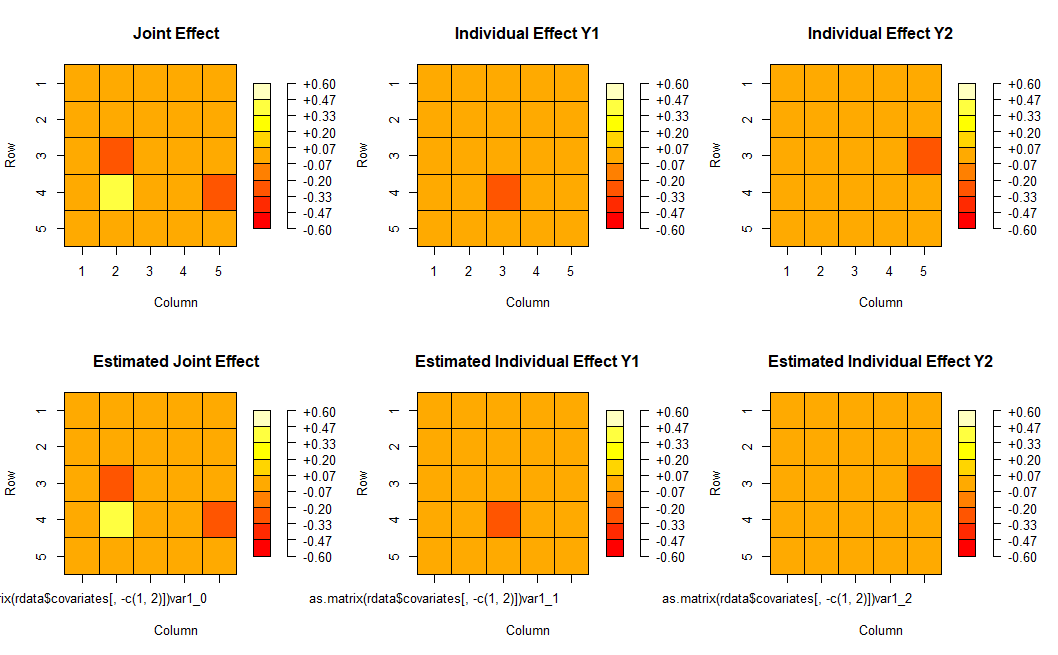
\includegraphics[width = \linewidth]{figures/2_VisRvarTrueEstPars}
		\caption{Illustration of the true and estimated Regression VAR parameters. For very large sample sizes, the traditional OLS method is successful. It would now be interesting to explore how regularization or model selection can help in higher dimension.}\label{fig:rvar_TrueEstimatedPars}
	\end{figure}
	
	\begin{figure}
		\centering
		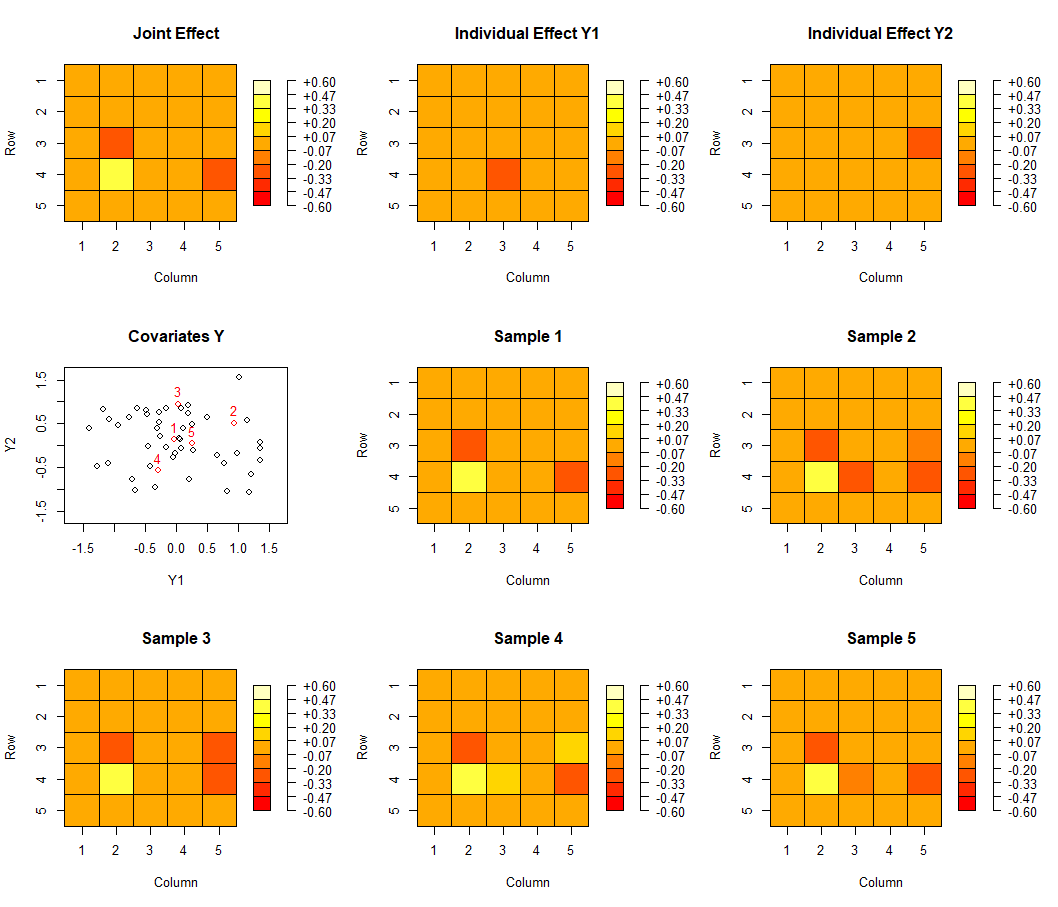
\includegraphics[width = \linewidth]{figures/1_VisParExample}
		\caption{Illustration of the Regression VAR framework with 2 covariate-dependent effects. Top-panels: visualization of the joint effects that are common across all subjects. We also visualize the effects that are individual to variables $X_1$ and $X_2$. Center-left panel: Visualization of the covariate information for $N = 50$ subjects. We highlight the covariate information of the first 5 subjects. Remaining panels: Visualization of the effects for the first 5 subjects. We observe that, as subject 1 has nearly zero for both $X_1$ and $X_2$, the effects are mostly just the joint effects. Subject 3 has a high $X_2$ covariate, but low $X_1$ covariate, and therefore its effects are a mixture of the joint and $X_2$ effects. Subject 2 has large covariates for both $X_1$ and $X_2$, so its time series effects are a mixture of all.}\label{fig:rvarCoeffsExample}
	\end{figure}
	
	
	\item For this same example, we performed a traditional LS fitting, to see if we could successfully recover the common/individual structure of the time series. As we see in Figure \ref{fig:rvar_TrueEstimatedPars}, our estimation for very large sample sizes is successful.
	

	
	
\end{itemize}

\newpage

\section{Fitting the RVAR Model with LASSO Penalty}\label{section:rvar}


In this section, we describe the fitting of the RVAR model of the form \eqref{eq:rvar}, with 1-lag relationships, \textit{i.e.} $q = 1$. Assuming that, for each individual $k=1,...,N$, we can capture the VAR relationships in matrix form as:
{\footnotesize
\begin{equation*}
	\underbrace{\begin{bmatrix} 
		(\bY_{T_k}^k)^{'} \\ (\bY_{T_k-1}^k)^{'} \\ \vdots \\ (\bY_{2}^k)^{'}
	\end{bmatrix}}_{\Zb^{k}} = 
	\underbrace{\begin{bmatrix} 
		(\bY_{T_k-1}^{k})^{'}  & X_{k1} (\bY_{T_k-1}^{k})^{'} &  X_{k2} (\bY_{T_k-1}^{k})^{'} & \ldots & X_{kp} (\bY_{T_k-1}^{k})^{'} \\
		(\bY_{T_k-2}^{k})^{'}  & X_{k1} (\bY_{T_k-2}^{k})^{'} &  X_{k2} (\bY_{T_k-2}^{k})^{'} & \ldots & X_{kp} (\bY_{T_k-2}^{k})^{'} \\
		 \vdots      &     \vdots      & \ddots & \vdots 		  \\
		(\bY_{1}^{k})^{'}  & X_{k1} (\bY_{1}^{k})^{'} &  X_{k2} (\bY_{1}^{k})^{'} & \ldots & X_{kp} (\bY_{1}^{k})^{'} \\
	\end{bmatrix}}_{\Wb^k} 
	\underbrace{\begin{bmatrix}
		\Psi_{0}^{'} \\ \Psi_{1}^{'} \\ \vdots \\ \Psi_{p}^{'}
	\end{bmatrix}}_{\Psi} +  
	\underbrace{\begin{bmatrix} 
		(\varepsilon_T^{k})^{'} \\ (\varepsilon_{T-1}^{k})^{'} \\ \vdots \\ (\varepsilon_{T-q+1}^{k})^{'}
	\end{bmatrix}}_{\Eb^{k}}.
\end{equation*}
}%
This can be simplified to matrix form as
\begin{equation}\label{eq:rvar_kmat}
	\Zb^{k} = \Wb^{k} \bPsi + \Eb^{k}
\end{equation}
The equation \eqref{eq:rvar_kmat} represents the VAR relationships for individual $k$. Then, we can model the behavior for all individuals via the equation
\begin{equation}\label{eq:multiresponse_regression}
	%\underbrace{\begin{bmatrix}  \Zb^1 \\ \Zb^2 \\ \vdots \\  \Zb^k \\ \vdots \\ \Zb^N \end{bmatrix}}_{\Zb} = 
	\underbrace{\begin{bmatrix}  \Zb^1 \\ \Zb^2  \\ \vdots \\ \Zb^N \end{bmatrix}}_{\Zb} = 
	%\underbrace{\begin{bmatrix}  \Wb^1 \\ \Wb^2 \\ \vdots \\  \Wb^k \\ \vdots \\ \Wb^N \end{bmatrix}}_{\Wb}  
	\underbrace{\begin{bmatrix}  \Wb^1 \\ \Wb^2  \\ \vdots \\ \Wb^N \end{bmatrix}}_{\Wb}  
	\bPsi + 
	%\underbrace{\begin{bmatrix}  \Eb^1 \\ \Eb^2 \\ \vdots \\  \Eb^k \\ \vdots \\ \Eb^N \end{bmatrix}}_{\Eb} 
	\underbrace{\begin{bmatrix}  \Eb^1 \\ \Eb^2 \\ \vdots \\ \Eb^N \end{bmatrix}}_{\Eb} ,
\end{equation}
Thus, we can summarize the VAR equation model for all individuals simultaneously with the reduced matrix equation:
\begin{equation}\label{eq:rvar_mat}
	\Zb = \Wb \bPsi + \bE,
\end{equation}
where $\Zb \in \bbR^{(T - N)\times d}$, $T = \sum_{k} T_k$, $\Wb\in \bbR^{(T - N)\times (d(p + 1))}$ and $\Eb \in \bbR^{(T - N)\times d}$. 

To solve for the parameter $\bPsi\in\bbR^{d (p+1) \times d}$, we propose the following optimization problem,
\begin{equation}\label{eq:rvar_matreg_lasso}
	\bhat\bPsi := \bhat\bPsi(\lambda_1,\lambda_2) = \argmin_{\bPsi\in \bbR^{d (p+1) \times d}} \vertiii{ \Zb - \Wb \bPsi }_{F}^2 + \lambda_1 \vertiii{\Psi_{0}}_1 +  \lambda_2 \vertiii{[\Psi_1 \, \Psi_2 \, \ldots \, \Psi_p]}_1,
\end{equation}
where the hyperparameter $\lambda_1$ serves to penalize the common structure of all VAR models, and $\lambda_2$ penalizes the $X$ covariate dependent portion of the model. We can interpret \eqref{eq:rvar_matreg_lasso} as a matrix regression problem. Notice that the optimization problem \eqref{eq:rvar_matreg_lasso} is equivalent to solving the separate column-wise optimization problems
\begin{equation}\label{eq:rvar_opt}
	\bhat\bPsi^{\ell}(\lambda_1,\lambda_2) = \argmin_{\bPsi^{(\ell)} \in \bbR^{d (p+1)}} \vertiii{ \Zb_{\cdot \ell} - \Wb \bPsi^{(\ell)} }_{F}^2 + \lambda_1 \|{[\bPsi^{(\ell)}]_{1:d}}\|_1 +  \lambda_2 \|{[\bPsi^{(\ell)}]_{(d+1):(dp)}}\|_1.
\end{equation}
When solving the individual optimization problems \eqref{eq:rvar_opt}, we can set the estimated parameter $\bhat\bPsi(\lambda_1,\lambda_2) := \left[\bhat\bPsi^{1}\, \bhat\bPsi^{2}\,\ldots \, \bhat\bPsi^{d}\right](\lambda_1,\lambda_2)\in\bbR^{d(p+1)\times d}$. Figure \ref{fig:rvar_TrueEstimatedPars} in the previous section was derived with $\lambda_1 = \lambda_2 = 0$.

The current implementation only allows for a single lagged relationship, \textit{i.e.} $q = 1$. We aim to create a more general implementation with lag $q> 1$ in the future. Alternatively, we can further vectorize the representation \eqref{eq:rvar_mat} into a single-response linear regression of the form 
\begin{align*}
	\bvec(\bZ) =  ( I_d \otimes  \Wb )  \cdot \bvec(\Psi) + \bvec(\Eb)
\end{align*}
where $\bvec(\Ab) = [A_{\cdot 1}^\mt , A_{\cdot 2}^\mt ,  \ldots A_{\cdot n}^\mt]^\mt\in\bbR^{ab}$ and $\Ab \otimes \Bb = [A_{ij}\cdot \Bb]_{i,j}\in\bbR^{ac \times bd}$ for any $\Ab\in\bbR^{a\times b}$ and $\Bb \in \bbR^{c\times d}$. Thus, solving \eqref{eq:rvar_opt} is equivalent to solving a weighted-penalty version of the LASSO \jose{add LASSO/glmnet ref}.

\subsection{Adaptive CD-VAR}\label{subsec:adaptiveCDVAR}

To improve upon the performance of our original estimator, we propose a refinement of our CD-VAR estimator through an adaptive approach. For this, let $\bhat{\bPsi}$ be an initial estimator of the CD-VAR model. Then, given a constant $\gamma > 0$ we define the adaptively-weighted $\ell_1$ penalty as:
\begin{equation}
	P_{ada}(\bPsi)  = \sum_{\ell = 1}^{p}\sum_{i, j=1}^{d}  |\Psi^{(\ell)}_{ij}|^{-\gamma}\cdot |\bPsi^{(w)}_{ij}|
\end{equation}
Then, for $\lambda >0$, our adaptive CD-VAR estimator is given as a solution to the optimization problem
\begin{equation*}\label{eq:rvar_opt}
	\bhat\bPsi_{ada}(\lambda_a) = \argmin_{\bPsi \in \bbR^{d \times (d(p+1))}} \vertiii{ \Zb - \Wb \bPsi }_{F}^2 + \lambda_a P_{ad}(\bPsi).
\end{equation*}

In following sections, we explore how the adaptive approach can help improve the edge-recovery performance. 


\subsection{Tuning Parameter Selection}

One of the main concerns when fitting a penalized model is to determine the best procedure for selecting tuning parameters. In particular, due to the dependence present in time series data, direct sample splitting is not feasible, leading to sophisticated procedures of data splitting to obtain a reasonable cross-validation procedure. For example \jose{add references, and what they do.}

\subsubsection{Cross-Validation}

Contrary to other methods like GIMME and Multi-VAR, one can generate ``predictive model coefficients'': with a model $\hat\bPsi\in\bbR^{d\times (p(d+1))}$ trained on the data of $N$ individuals $\{(\bX_k, \Yb^{(k)})\}_{k=1}^N$, we may provide an estimate of the coefficients of an out-of-sample individual $\{(\bX_{N+1}, \Yb^{(N+1)})$ via $\hat\Phi_{N+1} = \hat\Psi_{0} + \sum_{i=1}^p X_{ki} \hat\Psi_{i}$.

In our particular modeling, due to the independence across individuals, it is possible for us to perform cross validation as follows. Given a number of subjects $N$ and number of folds $K< N$, we divide the set of individuals $\{1,2,\ldots, N\} $into $K$ groups $\cG_1,\ldots, \cG_K$. Then, for each $k\in[K]$, the $k$-th fold consist of the union of all the data corresponding to the individuals in $\cG_k$. 

While simple, this approach for cross-validation cannot be used in usual VAR models, or even the Multi-VAR and GIMME methods. The main reason is that our model assumes a structural relationship between the exogenous covariates and the individual time-series model. Therefore, the training on a set of individuals $\cG\subset [N]$ can be used to infer the time-series coefficients for a new individual $i\in [N] \setminus \cG$. In contrast, methods like GIMME, Multi-VAR and their extensions must train individual coefficients for each individual separately. Therefore, fitting the time-series models for a subset of individuals $\cG\subset [N]$ cannot be exploited to determine the coefficients of a new individual $i\in [N] \setminus \cG$, or at least not directly.

On our case, since we assume that there is an underlying additive structure that connects all the individual time-series models, it is possible to train both the invidiual and common structure simultaneously. 


\subsubsection{BIC}

In addition to cross-validation, we alternatively propose the fitting of our model by selecting the tuning parameter that minimizes the Bayesian information criteria (BIC). Given $\lambda_1,\lambda_2 > 0$, we define,
\begin{equation}\label{eq:bic}
	\BIC(\lambda_1,\lambda_2) =  \vertiii{ \Zb - \Wb \bhat\bPsi(\lambda_1,\lambda_2) }_{F}^2 + \vertiii{\bhat\bPsi(\lambda_1,\lambda_2)}_0 \log(T-N)  . 
\end{equation}

Through numerical results, we have verified that BIC is a measure that leads to more sparse estimates of the matrix $\bPsi$ when compared to the estimate obtained through cross-validation.

\section{Fitting RUSEM}


The implementation of the RVAR model described in Section \ref{section:rvar} is simply a generalization of the optimization problem considered in the \citet{fisher2022penalized}. Notice that the RVAR focuses the estimation on the lagged effects $\bPsi$. For the GIMME model, we are also interested in recovering contemporaneous effects. The GIMME model cannot easily be extended to the regression setting. Therefore, we need to explore a different procedure for recovering the USEM structure in the regression setting. This will require thought and research...

I explored the original GIMME reference \citet{gates2012group}, which points towards the modification index described in \citet{sorbom1989model}. I am still trying to understand how the GIMME adapts the estimation of USEM described in \citet{sorbom1989model} to scenarios with time dependence. This will be the next task.




\section{Simulation Study for R-VAR}

To explore the performance of our proposed RVAR model, and to compare to other methods found in the literature, we perform a numerical simulation study.

\subsection{Simulation Setup}



We consider multivariate time series over $d = 10, 20, 30$ variables of interest. We consider scenarios with $N = 10, 20$ subjects, measured over $T = 30, 50, 100$ time points. For each subject $k\in\{1,2,\ldots , N\}$, we simulate a vector of $p = 2,5$ time-invariant covariates according to the mixture distribution $\bX_{k} = (X_{k1},X_{k2},\ldots , X_{kp})\stackrel{i.i.d.}{\sim} 0.25\cdot \delta_{0} + 0.75\cdot\Unif([-1,-0.5]\cup [0.5,1])$. Then, we simulate a lag-1 time series dataset for the subject $k \in \{1,2,\ldots , N\}$ according to the covariate-dependent VAR model \eqref{eq:rvar} with parameter $\bPsi(\bX_i)$, where 
\begin{equation*}
	\bPsi(\bx) = \Psi_0 + x_1 \Psi_1 + x_2 \Psi_2 + \ldots + x_p \Psi_p.
\end{equation*}
Finally, the common effect matrix $\Psi_0\in\bbR^{d\times d}$ and the matrix of covariate-dependent effects $\Psi_1,\ldots,\Psi_p \in\bbR^{d\times d}$ are generated as follows. First, we select the proportion of common non-zero entries $\eta_{c}$, a proportion of covariate-dependent non-zero entries $\eta_{i}$. We generate $\Psi_0$ by selecting at random $d^2 \eta_{c}$ entries to follow the distribution $\Unif([-0.9,-0.3]\cup[0.3,0.9])$. To generate $\Psi_k$,  we select $d^2 \eta_{i}$ to follow $\Unif([-0.9,-0.3]\cup[0.3,0.9])$. In our simulations, we consider $(\eta_c, \eta_i) = \{ (0.075,0.025), (0.025,0.075)\}$. Finally, we generate time series for the $k$-th subject $\{\bY^{(k)}_1,\bY^{(k)}_2,\ldots,\bY^{(k)}_{T+400}\}$ via the model \eqref{eq:rvar}, with $\be^{(k)}_1, \be^{(k)}_2, \ldots, \be^{(k)}_T\stackrel{i.i.d.}{\sim} N_{d}(\bzero, (0.1) \Ir_{d})$, and discard the first 400 time steps. 

We compare our proposed sparse CD-VAR method with methods of multi-subject vector auto-regressive models found in the literature. In particular, we consider the estimation of the time series via the individual VAR model \citep{basu2015regularized}, as well as the Multi-VAR method in their original and adaptive versions \citep{fisher2022penalized}. For the selection of the tuning parameters of the CD-VAR method, we consider training based on cross-validation, as well as based on our proposed BIC measure. Furthermore, we fit our method with both a direct and two-step adaptive approach, as described in Section \ref{subsec:adaptiveCDVAR}. 

We compare the methods in terms of several measurements of performance. First, we consider the mean root aggregated error (MRAE), and mean absolute aggregated error (MAAE), given by,
\begin{align*}
	MRAE &= \frac{1}{N}\sum_{k=1}^N  \sum_{\ell = 1}^p  \vertiii{\hat\Psi^{k}_{\ell} - \Psi^{k}_{\ell}}_F;\\
	%%
	MAAE &= \frac{1}{N}\sum_{k=1}^N  \sum_{\ell = 1}^p  \left\|\hat\Psi^{k}_{\ell} - \Psi^{k}_{\ell}\right\|_1;\\
\end{align*}



\subsection{Simulation Results}


The results of the MRAE for $d = 30$ are presented in Figure \ref{fig:30mrae}. The best performance for all scenarios is obtained by the adaptive CV-SCDVAR model, closely followed by the original CV-SCDVAR model and the adaptive BIC-SCDVAR model. This findings are consistent across choices of number of explanatory covariates $p=2,5$, number of subjects $N = 10, 20$, common entries $p_c = 0.025, 0.075$ and number of available time points $T$.  


\begin{figure}[h]
	\centering
	\includegraphics[width=0.9\textwidth, page=4]{sims_4/621_ByPnN_d30_sigma2_0.1.pdf}
	\includegraphics[width=0.9\textwidth, page=4]{sims_4/621_ByPnN_d20_sigma2_0.1.pdf}
	\caption{This is the caption for the inserted PDF page.}
	\label{fig:30mrae}
\end{figure}

\newpage

\end{comment}







\newpage


\begin{comment}
\section{Studying Consistency of VAR}


In order to show the consistency of our CD-VAR procedure, we must first explore and understand the consistency of the plain penalized VAR model. For this, we consider a sequence $\{\bX_t\}_{t\in\bbZ}\in\bbR^d$ distributed as a VAR($q$) model of the form:
\begin{equation}
    \bX_t = \sum_{\ell = 1}^q \Psi_\ell \bX_{t-\ell} + \varepsilon_t,
\end{equation}
where $\Psi_1,\Psi_2,\ldots ,\Psi_q \in \bbR^{d\times d}$ are the coefficient matrices. We first define the polynomial $\cA(z) = \Ir_d - \sum_\ell \Psi_\ell z^\ell $ for any $z\in\bbC$. To satisfy the stability condition, we need that $\det(\cA(z))\neq 0$ for all $z\in\bbC$ with $|z|\leq 1$. 

We define the auto-correlation matrices $\Gamma_X(i) = cov(X_
{t-i},X_t )$. Furthermore, we define the spectral density of the process as:
\begin{equation}
    f_X(\theta) = \frac{1}{2\pi} \sum_{\ell = -\infty}^{\infty} \Gamma_X(\ell) e^{-i\ell \theta},\hspace{5mm} \forall\, \theta\in[-\pi,\pi]. 
\end{equation}
Finally, we define the maximum spectral eigenvalue as,
\begin{equation}
    \cM(f_X) = \sup_{\theta\in[-\pi,\pi]} \Lambda_{\max} (f_X(\theta)) <\infty.
\end{equation}
Furthermore, for any $k$ we can define the sub-variable spectral density radius as,
\begin{equation}
    \cM(f_X,k) = \max_{\cJ\subset[d];\, |\cJ| = k} \cM(f_{X_\cJ})
\end{equation}
Similar to the spectral density radius, we can define the mimimum spectral density radius as:
\begin{equation*}
    m(f_X) = \inf_{\theta \in [-\pi,pi]} \Lambda_{\min} (f_X(\theta)).
\end{equation*}

There are several important observations:

\begin{itemize}
    \item The existence of the spectral density guarantees that 
    \begin{equation}
        \Gamma_X(\ell) = \int_{-\pi}^\pi f_X(\theta) e^{i\ell \theta}d\theta, \hspace{5mm} \forall\, \ell \in\bbZ.
    \end{equation}

    \item The spectral density radius $\cM(f_X)$ provides a measurement of the degree of dependence present in the data. If there is low dependence, then each of the terms $\|\Gamma_X(\ell)\|$ will decay fast for large $\ell$, so the eigenvalue $\Lambda_{\max}(f_X(\theta))$ will be small. If there is high dependence, then the terms $\|\Gamma_{X}(\ell)\|$ will stay large and the eigenvalues $\Lambda_{\max}(f_{X}(\theta))$ will remain large.

    \item We have that:
    $$ \cM(f_X, 1)\leq \cM(f_X, 1)\leq \ldots \leq \cM(f_X, d) = \cM(f_X).$$
\end{itemize}

Lets write down some useful facts.

Let $\Xb = [\bX_1,\bX_2, \ldots \bX_n]^{'} \in\bbR^{n\times d}$ be the matrix of observations from our time series, and $vec(\Xb) = [\bX_1^{'},\bX_2^{'}, \ldots \bX_n^{'}]^{'}\in\bbR^{nd}$. Let $\Upsilon^{X}_n = cov(vec(\Xb))\in \bbR^{nd\times nd}$. In particular, we have that
\begin{equation}
    \Upsilon^X_n = \begin{pmatrix}
        \Gamma_X(0) & \Gamma_X(1) & \dots & \Gamma_X(n) \\
        \Gamma_X(-1) & \Gamma_X(0) & \dots & \Gamma_X(n - 1) \\
        \vdots & \vdots & \ddots & \vdots \\
        
        \Gamma_X(-n) & \Gamma_X(-n+1) & \dots & \Gamma_X(0) \\
    \end{pmatrix}\in\bbR^{nd\times nd}.
\end{equation}

First, we can show that the spectra of the covariance $\Upsilon^X_n$ is bounded by the spectral density.


\begin{prop}[Proposition 2.3 of \ref{basu2015regularized}]
    For any $n\geq 1$ and $d \geq 1$,
    $$ 2\pi m(f_X) \leq \Gamma_{\min} (\Upsilon^X_n) \leq \Gamma_{\max}(\Upsilon^X_n) \leq 2\pi \cM(f_X) ; $$
    and in particular,
    $$ 2\pi m(f_X) \leq \Gamma_{\min} (\Lambda_X(0)) \leq \Gamma_{\max}(\Lambda_X(0)) \leq 2\pi \cM(f_X) . $$
\end{prop}
\begin{proof}
    Observe that for any $\bv\in\bbR^{nd}$ with $\|\bv\|=1$, and $\bv = [\bv_1^{'}, \ldots, \bv_n^{'}]^{'} \in\bbR^{nd}$, we have that for $G(\theta) = \sum \bv_i e^{-ir\theta}$,
    \begin{align*}
        \int_{-\pi}^\pi G^*(\theta)G(\theta)d\theta = \sum_{r,s} \int_{-\pi}^\pi v_s^{'}v_r e^{i(r-s)\theta}d\theta = \sum_r 2\pi\|\bv_r\|^2_2  = 2\pi
    \end{align*}
    On the other hand,
    \begin{align*}
        \bv^{'} \Upsilon^X_n \bv &= \sum_{r,s} \bv_s^{'} \Gamma_X(s-r) \bv_r\\
        %%
        &= \sum_{s,r} \int_{-\pi}^\pi \bv_s^{'}  f_X(\theta) \bv_r e^{i(s-r)\theta} d\theta\\
        %%
        &= \int_{-\pi}^\pi   G^*(\theta)  f_X(\theta)  G(\theta)d\theta.
        %%
    \end{align*}
    Finally, notice that for any $\theta\in[-\pi,\pi]$
    \begin{align*}
       & m(f_X)G^*(\theta) G(\theta) \leq G^*(\theta)  f_X(\theta)  G(\theta) \leq  \cM(f_X)G^*(\theta) G(\theta),\\
       %%
       \therefore \hspace{5mm}& 2\pi \cdot m(f_X) \leq  \Lambda_{\min}(\Upsilon^X_n) \leq  \Lambda_{\max}(\Upsilon^X_n) \leq 2\pi \cdot \cM(f_X).
    \end{align*}
\end{proof}


Furthermore, we consider the following sub-matrix concentration inequality. Let $S = \Xb^{'}\Xb / n$. We want to study how the matrix $S$ concentrates around $\Gamma_X(0)\in\bbR^{d\times d}$.

\begin{prop}[Proposition 2.4 of \ref{basu2015regularized}]
    For a stationary centered process $\Xb$ and $k$-sparse vectors $\bv,\bu\in\bbR^d$ with $\|\bv\| = \|\bu\| = 1$,
    \begin{align}
        &\bbP[|\bv^{'}  (S - \Gamma_X(0)) \bv| > 2\pi \cM(f_X, k) \eta] \leq 2\exp\{ -cn\min\{\eta^2,\eta\}  \},
        \label{eq:conc1}\\
        %%
        %%
        &\bbP[|\bu^{'}  (S - \Gamma_X(0)) \bv| > 2\pi \cM(f_X, 2k) \eta] \leq 6\exp\{ -cn\min\{\eta^2,\eta\}  \},\\
        %%
        %%
        &\bbP[|S_{ij} - [\Gamma_X(0)]_{ij}| > 2\pi \cM(f_X, 2) \eta] \leq 6\exp\{ -cn\min\{\eta^2,\eta\}  \}\,
    \end{align}
\end{prop}
\begin{proof}
    Lets just show \eqref{eq:conc1} first. Let $\cJ$ be the support of $\bv$. Observe that $vec(\Xb) \sim N_d(\bzero, \Upsilon^X_n )$. Then $vec(\Xb_J) \sim N_d(\bzero, \Upsilon^{X_{\cJ}}_n )$. From this $Y = \Xb \bv = \Xb_{\cJ} \bv_{\cJ}\in\bbR^{n}$. Then, we have $$cov(Y_r,Y_s) = cov( [\Xb_{\cJ}\bv_{\cJ}]_r, [\Xb_{\cJ}\bv_{\cJ}]_s ) = cov( \bX_r^{'} \bv , \bX_s^{'} \bv ) = \bv^{'}  cov( \bX_r , \bX_s ) \bv = \bv^{'} \Gamma_X(r-s) \bv.$$
    Thus, $\bY \sim N_n(\bzero, \Qr)$ with $\Qr_{rs} =  \bv^{'} \Gamma_X(r-s) \bv.$. Then, with $\bv^{'} S\bv = \frac{1}{n} \bY^{'} \bY = \frac{1}{n} \bZ^{'} \Qr \bZ$ where $\bZ \sim N_n(\bzero, \Ir_n)$.
    By the Hanson-Wright inequality, (Rudelson \& Vershynin, 2013) we have that:
    \begin{align*}
        \bbP[|\bv^{'} (S - \Gamma_X(0)) \bv| \geq \zeta] &= \bbP[|\bZ\Qr\bZ - \bbE[\bZ\Qr\bZ]| \geq n\zeta]  \\
        %%
        &\leq 2\exp\left\{  -cn\min\left[  \frac{n^2\zeta^2}{\vertiii{\Qr}_F^2} , \frac{n\zeta}{\vertiii{\Qr}_2} \right]  \right\}.
    \end{align*}
    Since $\vertiii{\Qr}_F^2 /n \leq \vertiii{\Qr}_2^2$, and setting $\zeta = \vertiii{\Qr}_2 \eta$, we have:
    \begin{equation}\label{eq:hansonwright_inter}
         \bbP[|\bv^{'} (S - \Gamma_X(0)) \bv| \geq \eta\vertiii{\Qr}_2] 
         %%
         \leq 2\exp\left\{  -cn\min[  \eta^2, \eta ]  \right\}.
    \end{equation}
    Finally, we observe that for $\bw \in\bbR^n$, and $\bW = [ w_1\bv^{'}_{\cJ} , w_2\bv^{'}_{\cJ} ,\ldots,  w_n\bv^{'}_{\cJ} ]^{'}$
    \begin{align*}
        \bw^{'} \Qr\bw &= \sum_{s,r} \bw_s\bw_r Q_{s,r} = \sum_{s,r} \bw_s\bw_r \bv^{'}_{\cJ} \Gamma_{X_{\cJ}}(r-s) \bv_{\cJ}\\
        %%
        &= \bW^{'} \Upsilon^{X_\cJ}_n \bW \leq \Lambda_{\max}(\Upsilon^{X_\cJ}_n) \leq 2\pi\cM(f_X, k)
    \end{align*}
    Thus, we can subsitute $\vertiii{\Qr}_2$ by $2\pi\cM(f_X, k)$ in \eqref{eq:hansonwright_inter}.
\end{proof}

\newpage

\end{comment}



	


\section{Consistency of MOD-VAR}

\subsection{Setting and Assumptions}

Consider observations on $n$ subjects, with vector of $p$ moderators $\bX_1,  \bX_2,\ldots \bX_n \in \bbR^p$ random vectors with $\bbE[\bX_k] = 0$ and entrywise bounded support: $|X_{ki}|\leq B$. We consider  $\Phi^{*(0)}, \Phi^{*(M1)}, \ldots, \Phi^{*(Mp)} \in \bbR^{d\times d}$  be the true model parameters, and we define $\Phi^* :\bbR^p \to \bbR^{d\times d}$ via the mapping $\Phi^*(\bx) = \Phi^{*(0)} + \sum_{s = 0}^p x_i\Phi^{*(Ms)} $. For each subject $k\in[n]$, we have $T$ measurements of a $d$-dimensional time-series $\{\bY^{(k)}_t \,:\, 1\leq t\leq T\}$, with the distribution:
\begin{equation}\label{eq:mod_var_vec}
    \bY^{k}_t = \Phi^*(\bX_k) \bY^{k}_{t-1} + \bvarepsilon_{t}^{k}, \hspace{5mm} \forall\, 2\leq t\leq T,    
\end{equation}
where $\bvarepsilon^{(k)}_2, \bvarepsilon^k_2, \ldots ,\bvarepsilon^k_T\stackrel{i.i.d.}{\sim}  N_d(\bzero, \Sigma_\varepsilon)$.
We denote:
\begin{equation}
    \Zb^{k} = \begin{pmatrix}
        (\bY^{k}_T)'\\ (\bY^{k}_{T-1})'\\ \vdots \\(\bY^{k}_{2})'\\ 
    \end{pmatrix}, \hspace{7mm}
    \Yb^{k} =  \begin{pmatrix}
        (\bY^{k}_{T-1})'\\ (\bY^{k}_{T-2})'\\ \vdots \\(\bY^{k}_{1})'\\ 
    \end{pmatrix}, \hspace{7mm}
    \Eb^{k} =  \begin{pmatrix}
        (\bvarepsilon^{k}_{T})'\\ (\bvarepsilon^{k}_{T-1})'\\ \vdots \\(\bvarepsilon^{k}_{2})'\\ 
    \end{pmatrix}.
\end{equation}
Thus, we can summarize the autoregressive structure for each subject given by \eqref{eq:mod_var_vec} via the matrix form equation:
\begin{equation*}
    \Zb^{k} = \Yb^{k} (\Phi^*(\bX_k))' + \Eb^{k}.
\end{equation*}
by a slight abuse of notation, we assume that for all $k\in[n]$, the vector of moderators $\bX_k\in\bbR^p$ contains a zero indexed entry $X_{k0} = 1$. We define $\Phi^* := [\Phi_0,\Phi_1,\ldots,\Phi_p]\in\bbR^{d\times (d+dp)}$, and 
\begin{equation*}
    \Wb^{k} = \left[\Yb^k , X_{k1}\Yb^k , \dots , X_{kp}\Yb^k \right] = \bX_k' \otimes \Yb^k \in \bbR^{(T-1) \times (d + pd)}.
\end{equation*}
Then, one can show that $\Yb^{k} (\Psi^*(\bX_k))' = \Wb^{k} (\Psi^*)'$. Now, we define
\begin{equation}
    \Zb = \begin{pmatrix}
        \Zb^{1}\\ \Zb^{2} \\ \vdots \\ \Zb^{n}
    \end{pmatrix}, \hspace{7mm}
    \Wb =  \begin{pmatrix}
        \Wb^{1} \\ \Wb^{2} \\ \vdots \\ \Wb^{n}  
    \end{pmatrix}, \hspace{7mm}
    \Eb =  \begin{pmatrix}
        \Eb^{1} \\ \Eb^{2} \\ \vdots \\ \Eb^{n} 
    \end{pmatrix}.
\end{equation}
Then, we can resume the entire model to our simplified matrix notation $\Zb = \Wb (\Phi^*)' + \Eb $.

For a matrix $\Ar = [\ba_1, \ba_2,\ldots \ba_m] \in \bbR^{k\times m}$ with column vectors $\ba_1,\ldots,\ba_m\in\bbR^{k}$, we denote $\bvec( \Ar) = (\ba_1', \ba_2',\ldots \ba_m')'\in\bbR^{km}$. Notice that,for any $\Phi \in \bbR^{d \times (d+dp)}$,
\begin{align*}
    \vertiii{\Zb - \Wb \Phi'}_F^2 &= \| \bvec(\Zb) - \bvec(\Wb\Phi') \|_2^2 = \|  \bvec(\Zb) - (\Ir_d \otimes \Wb)\bvec(\Phi')\|_2^2\\
    %%
    &= \bvec(\Zb)' \bvec(\Zb)  - 2 \bvec(\Zb)' (\Ir_d \otimes \Wb)\bvec(\Phi') +   \bvec(\Psi')'(\Ir_d \otimes \Wb'\Wb)\bvec(\Phi').
\end{align*}
To simplify our notation, we define $\bbeta = \bvec(\Phi')$, $\by = \bvec(\Zb)$, $\bgamma = \frac{1}{N} (\Ir_d \otimes \Wb')\by $ and $\hat\Gamma = \frac{1}{N} (\Ir_d \otimes \Wb' \Wb)$. In particular, we denote $\bbeta^* =\bvec((\Phi^*)')$. Finally, we denote $N = (T-1)n$ and $q = pd^2$. Then, assuming that $\lambda_2 = 0$, we can denote our proposed optimization problem:
\begin{equation}\label{eq:modvar_lasso_mat}
    \hat\Phi = \argmin_{\Phi\in \bbR^{d\times (d+dp)}} \frac{1}{N} \vertiii{ \bvec(\Zb) - \bvec(\Wb\Phi')}_F^2 + \lambda \vertiii{\Phi}_1
\end{equation}
into the equivalent form 
\begin{equation}\label{eq:modvar_lasso_vectorized}
    \hat\bbeta = \argmin_{\bbeta \in \bbR^{pd^2}} -2\bbeta ' \bgamma + \bbeta' \hat\Gamma\bbeta + \lambda \|\bbeta\|_1.
\end{equation}

First, we consider the following set of high-level assumptions. 

\begin{definition}[Restricted Eigenvalue]
    We say symmetric matrix $\Gamma\in\bbR^{q\times q}$ satisfies the restricted eigenvalue condition with parameters $\alpha,\tau > 0$ if for all $\btheta\in\bbR^q$, 
    \begin{equation}\label{eq:RE}
        \btheta' \hat\Gamma\btheta \geq \alpha \|\btheta\|_2^2 - \tau \|\btheta\|_1^2.
    \end{equation}
    We denote that a matrix $\Gamma\in\bbR^{q\times q}$ satisfies \eqref{eq:RE} as $\Gamma\in \RE(\alpha,\tau)$.
\end{definition}

\begin{assumption}\label{as:error_bound}
    There exists a function $Q(\bbeta^*, \Sigma_\varepsilon,B) >0$ such that,
    \begin{align*}
        \| \bgamma - \hat\Gamma \bbeta^* \|_\infty \leq Q(\bbeta^*, \Sigma_\varepsilon,B) \sqrt{\frac{2\log(d) + \log(p)}{N}}.
    \end{align*}
\end{assumption}


\begin{definition}[Conditional spectral Density]
    Assume $(\bX_k, \{ \bY^k_{t}\in\bbR^{d} \}_{t=1}^T)$ is a moderator vector autoregressive model, where $\{ \bY^k_{t}\in\bbR^{d} \}_{t=1}^T$ follows \eqref{eq:mod_var_vec}. We define the following.
    \begin{itemize}
        \item We define the \textit{conditional autocovariance function} as $\Gamma_{Y^k|X_k}(h) = \bcov(\bY^{k}_{t},  \bY^{k}_{t+ h}| \bX_k)$.
        %%
        %%
        \item We define the \textit{conditional spectral density function} as $$ f_{Y^k | X_k} (\theta) := \frac{1}{2\pi} \sum_{\ell = -\infty}^\infty \Gamma_{Y^k | X_k } (\ell) e^{-i\ell \theta}, \hspace{10mm} \theta\in [-\pi , \pi]. $$
        %%
        %%
        \item We denote the maximum spectral eigenvalue by 
        $$ \cM(f_{Y^k|X_k}) :=  \sup_{\theta\in[-\pi,\pi]} \Lambda_{\max} (f_{Y^k | X_k} (\theta)) .$$
        %%
        %%
        \item For any $\bx \in\bbR^p$, consider the matrix polynomial $\cA_{\bx}(z) = \Ir_d - \Phi^*(\bx) z $, for $z\in\bbC$. Then, we define the quantities:
        \begin{align}
            \mu_{\min}(\cA_{\bx})&:= \min_{|z| = 1} \Lambda_{\min} (\cA_{\bx}^*(z) \cA_{\bx}(z));\\
            %%
            %%
            \mu_{\max}(\cA_{\bx})&:= \max_{|z| = 1} \Lambda_{\max} (\cA_{\bx}^*(z) \cA_{\bx}(z)).
        \end{align}
    \end{itemize}
\end{definition}
    
\begin{definition}[$\alpha$-Orlicz norms]
    For a random variable $X\in\bbR$ and $\alpha > 0$, we define the $\alpha$-Orlicz norm  of $X$ as 
    \begin{equation*}
        \|X\|_{\psi_\alpha} := \inf\{ c > 0 \,:\, \bbE[\exp\{ |X|^\alpha/c^\alpha \}] \leq 2 \}.
    \end{equation*}
\end{definition}

\subsection{Useful Lemmas}




\begin{lemma}[Lemma 12 in \citet{loh2011high}]\label{lemma:badRE_to_goodRE}
    Let $\Gamma \in\bbR^{q\times q}$, $s\geq 1$ and $\delta > 0$. Suppose $\Gamma$ satisfies the deviation bound
    \begin{equation*}
       \sup_{\|\bv\|_2 = 1 ,\, \|\bv\|_0 \leq 2s} |\bv' \Gamma \bv| < \delta .
    \end{equation*}
    Then, for all $\bv\in\bbR^{q}$
    \begin{equation*}
        |\bv' \Gamma \bv| \leq 27\delta(\|\bv\|_2^2 + \frac{1}{s} \|\bv\|_1^2).
    \end{equation*}
\end{lemma}

\begin{lemma}[Lemma B.1 of \citet{basu2015regularized}] \label{lemma:re_kronecker}
    If $\Wb'\Wb / N \in \RE(\alpha,\tau)$, then the matrix $I_d \otimes \Wb'\Wb / N$ satisfies $I_d \otimes \Wb'\Wb / N \in \RE(\alpha,\tau)$ as well.
\end{lemma}



\begin{lemma}[Proposition 2.4 of \citet{basu2015regularized}]\label{lemma:ts_cov_concentration}
    Consider a centered Gaussian time series $\{Y_t\}_{t\in\bbZ}$ with noise matrix $\Eb\in\bbR^{(T-1) \times d}$ such that $\cM(f_{Y}) <\infty$. Let $\Yb = [\bY_1, \bY_2,\ldots \bY_T]'\in\bbR^{T\times d}$ and $\Eb = [\bvarepsilon_1,\bvarepsilon_2,\ldots ,\bvarepsilon_T]'\in\bbR^{T\times d}$.  There exists a constant $c>0$ such that, for any $s$-sparse vectors $\bv,\bu\in\bbR^p$ with $\|\bv\|_2 , \|\bu\|_2 \leq 1$, 
    $$\bbP\left[ |\bu' (\Yb' \Eb / T ) \bv| > 2\pi \Lambda_{\max}(\Sigma_\varepsilon) \left( 1 + \frac{1 + \mu_{\max}(\cA)}{\mu_{\min}(\cA)} \right) \eta \right] \leq 6 \exp\left[ - cn \min(\eta, \eta^2)\right].$$
\end{lemma}



\begin{lemma}[Exercises 2.24 and 2.44 of \citet{vershynin2018high}]
    Let $X\in\bbR$ a random variable with $\|X\|_{\psi_\alpha} <\infty$. Then,  there exists a constant $c > 0 $ such that,
    \begin{itemize}
        \item $\|X-\bbE X\|_{\psi_\alpha} \leq c\|X\|_{\psi_\alpha}$; and,
        \item if $|X| \leq B$, then $\|X\|_{\psi_\alpha} \leq c B$.
    \end{itemize}
\end{lemma}

\begin{lemma}[Theorem 3.4 of \citet{kuchibhotla2022moving}]\label{lemma:cov_conc_hetero}
    Suppose that $\bX_1, \bX_2,\ldots ,\bX_n \in\bbR^{q}$ are independent, mean-zero vectors such that, for some $\alpha > 0$ and $K_{n,q} , \eta_{n,q} > 0$, 
    \begin{equation}
        \max_{1\leq i\leq n} \max_{1\leq j\leq q} \|X_{ij}\|_{\psi_\alpha} \leq K_{n,q}, \hspace{10mm}  \max_{1\leq j \leq q} \frac{1}{n} \sum_{i=1}^n \bbE[X_{ij}^2] \leq \eta_{n,q}.
    \end{equation}
     Then, for any $t> 0$, with probability at least $1 - 3 e^{-t}$, 
    \begin{equation}
        \left\|\frac{1}{n} \sum_{i=1}^n X_i\right\|_{\infty} \leq 7\sqrt{ \frac{ \eta_{n,q} (\log(q) + t) }{n} } + \frac{C_\alpha K_{n,q} (\log(2n))^{1/\alpha} (\log(q) + t)^{1/\alpha^*} }{n},
    \end{equation}
    where $\alpha^* := \min\{1,\alpha\}$ and $C_\alpha > 0$ is some constant depending only on $\alpha$.
\end{lemma}

\begin{lemma}[Proposition D.2 of \citet{kuchibhotla2022moving}]
    Let $W_1,W_2,\ldots,W_k$ are possibly dependent random variables satisfying $\|W_i\|_{\psi_{\alpha_i}} <\infty$ for some $\alpha_i > 0$. Then,
    \begin{equation}
        \left\| \prod_{i=1}^k W_i \right\|_{\psi_\beta} \leq \prod_{i=1}^k \|W_i\|_{\psi_{\alpha_i}}, \hspace{10mm} where \quad \frac{1}{\beta} := \sum_{i=1}^k \frac{1}{\alpha_i}.
    \end{equation}
    
\end{lemma}

\subsection{Proof of Theorem \ref{thm:modvar_normconsistency}}

\begin{prop}
    Consider the MOD-VAR estimator $\hat\bbeta$ defined by \eqref{eq:modvar_lasso_vectorized}. Assume that $\hat\Gamma \in\RE(\alpha,\tau)$ for $s\tau < \alpha/32$. Furthermore, suppose Assumption \ref{as:error_bound} holds. Finally, assume that $$ \lambda \geq 4Q(\bbeta^*, \Sigma_\varepsilon, B) \sqrt{\frac{2\log(d) + \log(p)}{N}}.$$
    Then,
    \begin{align*}
        \|\hat\bbeta - \bbeta^* \|_2  \leq \frac{3\sqrt{s}\lambda}{\alpha} ; \hspace{10mm} \| \hat\bbeta - \bbeta^*\|_1 \leq \frac{12s \lambda}{\alpha}.
    \end{align*}
\end{prop}
\begin{proof}
    If $\hat\bbeta$ is the minimizer of \eqref{eq:modvar_lasso_vectorized}, 
    $$  -2\hat\bbeta' \bgamma + \hat\bbeta'\hat\Gamma\hat\bbeta + \lambda\|\hat\bbeta\|_1  \leq  -2(\bbeta^*)' \bgamma + (\bbeta^*)'\hat\Gamma\bbeta^* + \lambda\|\bbeta^*\|_1. $$ 
    By denoting $\bDelta = \hat\bbeta - \bbeta^*$, by basic manipulation and the triangle inequality,
    \begin{equation}\label{eq:step1}
        0\leq \bDelta' \hat\Gamma \bDelta  \leq 2\bDelta' ( \bgamma - \hat\Gamma \bbeta^* ) + \lambda\|\bDelta_{\cS}\|_1 - \lambda\| \bDelta_{\cS^c}\|_1.    
    \end{equation}
    By Assumption \ref{as:error_bound} and Hölder's inequality,
    \begin{equation}\label{eq:step2}
        2\bDelta' ( \bgamma - \hat\Gamma \bbeta^* ) \leq 2Q(\bbeta^*, \Sigma_\varepsilon, B) \sqrt{\frac{2\log(d) + \log(p)}{N}} \|\bDelta\|_1 \leq \frac{\lambda}{2} \|\bDelta\|_1.
    \end{equation}
    Combining \eqref{eq:step1} and \eqref{eq:step2}, we have the following two conclusions
    \begin{equation*}
        0\leq \frac{1}{\lambda}\bDelta' \hat\Gamma \bDelta  \leq \frac{3}{2}\|\bDelta_{\cS}\|_1 - \frac{1}{2}\|\bDelta_{\cS^c}\|_1 \leq  \frac{3}{2}\|\bDelta_{\cS}\|_1; \hspace{10mm} and,\hspace{10mm} \|\bDelta\|_1 \leq 4\|\bDelta_{\cS}\|_1.
    \end{equation*}
    Note that $\|\bDelta\|_1 \leq 4\|\bDelta_\cS\|_1 \leq 4\sqrt{s} \|\bDelta_\cS\|_2 \leq 4\sqrt{s} \|\bDelta\|_2$. Since $\hat\Gamma\in\RE(\alpha, \tau)$, we have that,
    \begin{align*}
        \bDelta'\hat\Gamma \bDelta\geq \alpha \|\bDelta\|_2^2 - \tau \|\bDelta\|_1^2 \geq \alpha \|\bDelta\|_2^2 - \frac{\alpha}{2}\|\bDelta\|_2^2 = \frac{\alpha}{2}\|\bDelta\|_2^2.
    \end{align*}
    Then, $$\frac{\alpha}{2} \|\bDelta\|_2^2 \leq \bDelta' \hat\Gamma \bDelta \leq \frac{3\lambda}{2}\|\bDelta_{\cS}\|_1 \leq \frac{3\sqrt{s}\lambda}{2} \|\bDelta\|_2.$$ 
    Thus, we conclude $\|\hat\bbeta - \bbeta^*\|_2 \leq 3\sqrt{s}\lambda / \alpha$. Furthermore, $\|\hat\bbeta - \bbeta^*\|_1 \leq 4\sqrt{s}\|\bDelta\|_2 \leq 12s \lambda/\alpha$.
\end{proof} 



\begin{prop}\label{prop:errorbound_whp}
    Assume that $N > 16\log(pd^2)$, and 
    \begin{equation}
        C_M := \sup_{\bx\in\bbR^p}  \Lambda_{\max}(\Sigma_\varepsilon) \left( 1 + \frac{1 + \mu_{\max}(\cA_x)} {\mu_{\min}(\cA_x)} \right) < \infty.
    \end{equation}
    Then, we have that,
    \begin{equation*}
        \bbP\left[ \|\bgamma - \hat\Gamma \bbeta^*\|_\infty  \geq 4\pi C_M B \sqrt{\frac{2\log(d) + \log(p)}{N}} \right] \leq 6\exp\{ -3c (2\log(d) + \log(p)) \}.
    \end{equation*}
\end{prop}
\begin{proof}
    First, observe that,
    \begin{align*}
        \bgamma &= \frac{1}{N} (\Ir_d \otimes \Wb') \bvec(\Zb) = \frac{1}{N} (\Ir_d \otimes \Wb'\Wb) \bvec({\Phi^{*}}') + \frac{1}{N}(\Ir_d \otimes \Wb') \bvec(\Eb);\\
        %%
        \hat\Gamma \bbeta^* &= \frac{1}{N} (\Ir_d \otimes \Wb'\Wb) \bvec({\Phi^{*}}').
    \end{align*}
    
    Thus, observe that,
    \begin{align*}
        \| \bgamma - \hat\Gamma \bbeta^* \|_\infty &= \|\bvec(\Wb'\Eb)/N\|_\infty = \vertiii{ \Wb'\Eb/N }_{\max} = \max_{\substack{1\leq i\leq p;\\ 1\leq m,\ell\leq d }} \left|  \frac{1}{n} \sum_{k=1}^n \frac{1}{T-1} X_{ki} (\bY^{k}_{\cdot m})' \bE^{k}_{\cdot \ell} \right|.
    \end{align*}
    By Lemma \ref{lemma:ts_cov_concentration}, there exists $c> 1$ such that for any $\eta > 0$,
    \begin{equation*}
        \bbP\left[  \left|\frac{1}{T-1}  (\bY^{k}_{\cdot m})' \bE^{k}_{\cdot \ell} \right|  \geq 2\pi C_M \eta \right] \leq 6 \exp\left\{  - c (T-1) \min(\eta,\eta^2) \right\}.
    \end{equation*}
    Recall that $|X_{ki}| \leq B$. Using this fact, and aggregating all the independent sub-exponential bounds, 
    \begin{equation*}
        \bbP\left[  \left|\frac{1}{n} \sum_{k=1}^n \frac{1}{T-1} X_{ki} (\bY^{k}_{\cdot m})' \bE^{k}_{\cdot \ell}  \right|  \geq t \right] \leq 6 \exp\left\{ -\min\left[  \frac{cNt^2}{4\pi^2 C_M^2 B^2}, \frac{cNt}{2\pi C_M B} \right] \right\}.
    \end{equation*}
    Notice that, if $N > 16\log(pd^2) $, and $t^* = 4\pi C_M B \sqrt{\log(d^2p)/N}$, 
    $$ \frac{cN(t^*)^2}{4\pi C_M B^2 } = 4c\log(pd^2) < 2c\sqrt{N \log(pd^2) }  = \frac{cNt^*}{2\pi C_M B}. $$
    Thus, 
    \begin{equation*}
        \bbP\left[  \left|\frac{1}{n} \sum_{k=1}^n \frac{1}{T-1} X_{ki} (\bY^{k}_{\cdot m})' \bE^{k}_{\cdot \ell}  \right|  \geq   4\pi C_M B \sqrt{\frac{\log(d^2p)}{N}}  \right] \leq 6 \exp\left\{ -4c\log(pd^2) \right\}.
    \end{equation*}
    By applying the union bound, we obtain,
    \begin{align*}
        \bbP\left[  \max_{\substack{1\leq i\leq p;\\ 1\leq m,\ell\leq d }} \left|\frac{1}{N} \sum_{k=1}^n  X_{ki} (\bY^{k}_{\cdot m})' \bE^{k}_{\cdot \ell}  \right|  \geq   4\pi C_M B \sqrt{\frac{\log(d^2p)}{N}}  \right] &\leq 6 \exp\left\{ \log(pd^2) -4c\log(pd^2) \right\} \\
        %%
        %%
        &\leq  6 \exp\left\{ -3c\log(pd^2) \right\} .
    \end{align*}
\end{proof}


\begin{prop}\label{prop:RE_ours}
    For any $t > 0$, consider 
    \begin{align*}
        \delta := \delta(t) &= 7\sqrt{\frac{\eta B^2 (\log(d^2p) + t)}{ n} } + \frac{ K B^2\log(2n)(\log(d^2p) + t) }{n},\\
        %%
        \Lambda_{Y} &:= \inf_{\bx} \Lambda_{\min} (\Gamma_{Y|\bx}(0)),\\
        %%
        \alpha^* &= \Lambda_{Y}\Lambda_{\min}(\Sigma_X) /2,\\
        %%
        \tau^* &= {54\delta}.
    \end{align*}
    Then, for all $t > 0$ such that $\alpha^* > 54s\delta$, we have that $\hat\Gamma = (\Ir_d \otimes \Wb'\Wb)/N \in\RE(\alpha^*,\tau^*)$ with probability at least $1- 3e^{-t}$.
\end{prop}
\begin{proof}
    First, by Lemma \ref{lemma:re_kronecker}, it suffices to show $\Wb'\Wb/N\in\RE(\alpha,\tau)$. We denote $\Sigma_W = \bbE[\Wb'\Wb/N]$. To achieve this, the steps will be as follows: (\textit{i}) show that $\bv' \Sigma_W \bv > K \| \bv\|_2^2$ for some constant $K>0$, (\textit{ii}) use Lemma \ref{lemma:cov_conc_hetero} to show that $|\bv'(\Wb'\Wb/N - \Sigma_W )\bv | = o_p(1)$, and (\textit{iii}) apply Lemma \ref{lemma:badRE_to_goodRE} to derive the restricted eigenvalue property for $\Wb'\Wb/N$ with probability at least $1 - 3e^{-t}$.
    
    First, we note that,
    \begin{align*}
        \frac{1}{N} \Wb'\Wb = \frac{1}{n} \sum_{k=1}^n \bX_k\bX_k' \otimes \left( \frac{1}{T-1} (\Yb^k)'\Yb^k  \right)
    \end{align*}
    Let $\Vr \in\bbR^{p\times d}$ be a matrix with columns $\Vr = [\bv_1,\bv_2,\ldots ,\bv_d]$. Let $\bv = (\bv_1',\bv_2',\ldots ,\bv_d')'\in\bbR^{pd}$. Then, observe that,
    \begin{align*}
        \Wb^k \bv &=  [\bX_k' \otimes \Yb^k] \bv = \sum_{a=0}^{p} x_{ka} \Yb^k \bv_a = \Yb^k \Vr \bX_k
    \end{align*}
    Using the same notation for $\Vr\in\bbR^{p\times d}$ and $\bv\in\bbR^{pd}$, we have that 
    \begin{align*}
        \bbE\left[ \frac{1}{N} \bv'\Wb' \Wb \bv \right] &= \frac{1}{N} \sum_{k=1}^n \bbE[  \bX_k'\Vr' (\Yb^k)' \Yb^k \Vr \bX_k] \\
        %%
        &= \bbE\left\{\bbE\left[  \frac{1}{n}  \sum_{k=1}^n  \bX_k'\Vr' \left(\frac{1}{T-1} (\Yb^k)' \Yb^k \right) \Vr \bX_k\big| \Xb \right]\right\}\\
        %%
        &= \bbE\left[  \bX_1'\Vr' \Gamma_{Y|X_1}(0) \Vr \bX_1 \right] \\
        %%
        &\geq \Lambda_{Y} \bbE\left[  \bX_1'\Vr' \Vr \bX_1 \right] \geq \Lambda_{Y} \Lambda_{\min}(\Sigma_{X}) \|\bv\|_2^2
    \end{align*}
    Now, we focus on providing concentration for $\sup_{\|\bv\|_0 \leq 2s;\, \|\bv\|=1} |\bv'(\Wb'\Wb/N - \Sigma_W )\bv |$. Note that,
    $$ \frac{1}{N} \Wb'\Wb = \frac{1}{n}\sum_{k=1}^n  (\Xb_k\Xb_k') \otimes \left(\frac{1}{T-1} (\Yb^k)'\Yb^k \right).$$
    Since the terms $\{(\Xb_k\Xb_k') \otimes [(\Yb^k)'\Yb^k] /(T-1) \}_{k=1,\ldots,n}$ are independent, we may apply Lemma \ref{lemma:cov_conc_hetero}. To this aim, observe that for any $1\leq i,j\leq d$ and $1\leq \ell,m \leq p$, by Lemma \ref{lemma:ts_cov_concentration},
    \begin{align*}
        \left|\left[\frac{1}{T-1} (\Xb_k\Xb_k') \otimes(\Yb^k)'\Yb^k \right]_{i\ell, jm} \right|&= \frac{1}{T-1}\left| X_{k\ell}X_{km} (\bY^{k}_{\cdot i})'\bY^{k}_{\cdot j}\right| \\
        %%
        &\leq \frac{B^2}{T-1}  \left|(\bY^{k}_{\cdot i})'\bY^{k}_{\cdot j}\right| \\
        %%
        &\leq  B^2\Gamma_{Y|X_k}(0)_{ij} + O_p\left( \frac{C_M B^2}{T-1}\right) = O_p(B^2).
    \end{align*}
    On the other hand, 
    \begin{align*}
        \max_{\substack{ 1\leq i,j\leq d \\ 1\leq \ell,m \leq p}} \frac{1}{n} \sum_{k=1}^n \bbE\left[ \left(\frac{1}{T-1} X_{k\ell}X_{km} (\bY^{k}_{\cdot i})'\bY^{k}_{\cdot j}\right)^2  \right] &= \max_{\substack{ 1\leq i,j\leq d \\ 1\leq \ell,m \leq p}} \bbE\left[ \left(\frac{1}{T-1} X_{1\ell}X_{1m} (\bY^{1}_{\cdot i})'\bY^{1}_{\cdot j}\right)^2  \right]\\ 
        %%
        &\leq \max_{\substack{ 1\leq i,j\leq d \\ 1\leq \ell,m \leq p}}  B^2 \bbE\left[ \left(\frac{1}{T-1} (\bY^{1}_{\cdot i})'\bY^{1}_{\cdot j}\right)^2  \right]\\
        %%
        &\leq O_p\left( B^2 \right)
    \end{align*}
    As a consequence, for appropriately chosen constants $K, \eta > 0 $, by Lemma \ref{lemma:cov_conc_hetero},
    \begin{equation*}
        \vertiii{ \frac{1}{T-1}\Wb'\Wb - \Sigma_W }_{\max} \leq \delta := 7\sqrt{\frac{\eta B^2(\log(d^2p) + t)}{ n} } + \frac{  KB^2 \log(2n)(\log(d^2p) + t) }{n}
    \end{equation*}
    with probability at least $1 - 3e^{-t}$. From this, it can easily be shown that,
    \begin{align*}
        \sup_{\substack{\|\bv\|_0 \leq 2s \,;\, \|\bv\|_2 = 1}} \left|\bv' \left(\frac{\Wb'\Wb}{N} - \Sigma_W \right) \bv\right| \leq 2s\delta.
    \end{align*}
    Applying Lemma \ref{lemma:badRE_to_goodRE}, it follows that, for any $\bv\in\bbR^{pd}$
    \begin{align*}
        \left|\bv' \left(\frac{\Wb'\Wb}{N} - \Sigma_W \right) \bv\right| \leq 54s\delta  \|\bv\|_2^2 + {54\delta} \|\bv\|_1^2.
    \end{align*}
    
    To conclude, observe that for any $\bv\in\bbR^{pd}$
    \begin{align*}
        \left|\bv' (\frac{1}{T-1} \Wb'\Wb)  \bv\right| &\geq  |\bv\Sigma\bv|  - \left|\bv' \left(\frac{\Wb'\Wb}{N} - \Sigma_W \right) \bv\right|\\
        %%
        &\geq (\Lambda_{Y}\Lambda_{\min}(\Sigma_X) - 54s\delta )\|\bv\|_2^2 - {54\delta}  \|\bv\|_1^2.  
    \end{align*}    
    Thus, as long as $\Lambda_{Y} \Lambda_{\min}(\Sigma_X) /2 > 54s\delta $, it follows that,
    $\Wb'\Wb/N \in RE(\alpha^*,\tau^*)$ for $\alpha^* = \Lambda_{Y}\Lambda_{\min}(\Sigma_X) /2$ and $\tau = {54\delta}$ and $\delta > 0$ is as defined above.
\end{proof}





\newpage
\begin{thm*}
    Consider the MOD-VAR estimator $\hat\Phi\in\bbR^{d\times (dp+d)}$ defined by \eqref{eq:modvar_lasso_mat}. Assume that $\Phi^*$ is $s$-sparse, \textit{i.e.} $\|\Phi^*\|_0 = s$, and we have equal sample size $T$ for all $n$ subjects. Let $N = n(T-1)$. Then, there exist universal constants $K,\eta , c > 0$ such that the following statements hold. Let $t>0$, and 
    \begin{align*}
        \delta&:= \delta(t) =  7\sqrt{\frac{\eta B^2(\log(d^2p) + t)}{ n} } + \frac{  K B^2\log(2n)(\log(d^2p) + t) }{n},\\
        %% 
        \Lambda_{Y} &:=  \inf_{\bx} \Lambda_{\min}(\Gamma_{Y|\bx}(0)),\\
        %%
        \alpha^* &:= \Lambda_{\min}(\Sigma_X) \Lambda_{Y} / 2, \\
        %%
        \tau^* &:= 54s\delta ,\\
        %%
        C_M &:= \sup_{\bx\in\bbR^p}  \Lambda_{\max}(\Sigma_\varepsilon) \left( 1 + \frac{1 + \mu_{\max}(\cA_x)} {\mu_{\min}(\cA_x)} \right) ,\\
        %%
        Q(\bbeta^*, \Sigma_\varepsilon, B) &:= 4B \pi C_M.
    \end{align*}
    Whenever the following inequalities are satisfied
    \begin{align}
        \alpha^* &> 32s \tau^*  \label{eq:thm1_re_cond} \\
        %%
        N &> 16\log(pd^2) \label{eq:thm1_errorbound_cond1}\\
        %%
        C_M &< \infty, \label{eq:thm1_errorbound_cond2}\\
        %%
        \lambda &> 4Q(\bbeta^*, \Sigma_\varepsilon, B) \sqrt{\frac{2\log(d) + \log(p)}{N}} \label{eq:thm1_lambda_cond}.
    \end{align}
    our MOD-VAR estimator satisfies the consistency 
    \begin{align*}
        \|\hat\Psi - \Psi^* \|_2  \leq \frac{24\sqrt{s} Q(\bbeta^*, \Sigma_\varepsilon, B)}{\Lambda_{Y}\Lambda_{\min}(\Sigma_X)}  \sqrt{\frac{2\log(d) + \log(p)}{N}};\\
        %%
        %%
        \| \hat\Psi - \Psi^*\|_1 \leq  \frac{144 s Q(\bbeta^*, \Sigma_\varepsilon, B)}{\Lambda_{Y} \Lambda_{\min}(\Sigma_X)}  \sqrt{\frac{2\log(d) + \log(p)}{N}}.
    \end{align*}
    with probability at least $1 - 3e^{-t} - 6e^{-3c\log(d^2p)}$.
\end{thm*}
\begin{proof}
    By \eqref{eq:thm1_re_cond}, we have $\alpha^* > 32s \tau^* > 108s\delta$. By Proposition \ref{prop:RE_ours} we have $\hat\Gamma \in\RE(\alpha^*,\tau^*)$ with probability at least $1 - 3e^{-t}$. 

    By \eqref{eq:thm1_errorbound_cond1}, \eqref{eq:thm1_errorbound_cond2}, and applying Proposition \ref{prop:errorbound_whp} we have that,
    $$  \|\bgamma - \hat\Gamma \bbeta^*\|_\infty  < Q(\bbeta^*, \Sigma_\varepsilon, B)\sqrt{\frac{2\log(d) + \log(p)}{N}} $$
    with probability at least $1 - 6\exp\{ -3c (2\log(d) + \log(p)) \}$. Therefore, Assumption \ref{as:error_bound} is satisfied.

    Furthermore, note that by \eqref{eq:thm1_lambda_cond}, $$ \lambda \geq 4Q(\bbeta^*, \Sigma_\varepsilon, B) \sqrt{\frac{2\log(d) + \log(p)}{N}}.$$

    Since the restricted eigenvalue condition is satisfied for $\alpha^* > 32 s \tau^*$, and Assumption \ref{as:error_bound} holds, we have that:
        \begin{align*}
        \|\hat\bbeta - \bbeta^* \|_2  \leq\frac{3\sqrt{s}\lambda}{\alpha}  =  \frac{24\sqrt{s} Q(\bbeta^*, \Sigma_\varepsilon, B)}{\Lambda_{Y} \Lambda_{\min}(\Sigma_X)}  \sqrt{\frac{2\log(d) + \log(p)}{N}};\\
        %%
        %%
        \| \hat\bbeta - \bbeta^*\|_1 \leq \frac{12s \lambda}{\alpha} =  \frac{144 s Q(\bbeta^*, \Sigma_\varepsilon, B)}{\Lambda_{Y} \Lambda_{\min}(\Sigma_X)}  \sqrt{\frac{2\log(d) + \log(p)}{N}}.
    \end{align*}
\end{proof}





\section{Additional Simulation Results}\label{supmat_section:add_sims}

As explored in Section \ref{section:simulations}, we present a comparison of performance of our proposed MOD-VAR for cases in which there is heterogeneity in the time series due to moderator effects, as well as a combination of moderator and fully individual effects. These comparisons focus on MSE and forecasting error. In the present section, we provide simulation comparisons of our proposed method in terms of mean true positive rate (TPR), mean false positive rate (FPR) and time performance. Additionally, we share simulation performance results for the scenario where heterogeneity is present, but it is fully individual, with no moderator effects.

In Section \ref{}

\subsection{True and False Positive Rates}\label{supmat_subsec:sims_tpr_fpr}




\subsection{Results for Fully Individual Heterogeneous Time Series}\label{supmat_subsec:sims_fully_individual}




\subsection{Computational Time}\label{supmat_subsec:sims_comp_time}







\bibliographystyle{apalike}
\bibliography{ref}

\end{document}
